{
\renewcommand\indexmarker{\cdot}


\chapter{Rappels de Relativité Restreinte}
La première partie de ce chapitre (section 1-4) est constitué exclusivement de rappels de la relativité restreinte. Celle-ci sera importante dans la suite du cours, comme elle reste valable \emph{localement} en présence de gravitation, dans un RLI. La seconde partie du chapitre (section 5-6) approfondit ces notions via une étude de la \emph{structure causale} de l'espace de Minkowski.


\section{Postulats de la relativité restreinte}
En 1905, Einstein énonça les deux postulats de la relativité restreinte:
\begin{theoremframe}
    \begin{post}[Loi de la relativité]
        Les lois de la physique prennent la même forme dans tous les référentiels inertiels. Il est donc impossible de distinguer un référentiel inertiel d'un autre.
    \end{post}
\end{theoremframe}
\begin{theoremframe}
    \begin{post}[Universalité de la vitesse de la lumière]
        La vitesse de la lumière $c$ dans le vide est isotope et prend la même valeur dans tout référentiel inertiel.
    \end{post}
\end{theoremframe}
\section{Définition d'un référentiel inertiel}

La relativité restreinte est une théorie de l'espace-temps plat quadri-dimensionnel $\R ^{1,3}$, dont les points sont appelés des \emph{événements}. Les \emph{référentiels} permettent d'enregistrer ces événements, et sont constitués de:
\begin{enumerate}
    \item un repère spatial cartésien orthonormé au repos de coordonnées $(x, y, z) = \vect{x}$, souvent écrit en composantes $x^k$ où $k=1, 2, 3$. 
    \item des horloges qui déterminent quand l'événement a lieu $x^0 = ct$. \\
\end{enumerate}
Un point $x^\mu\in \R^{1,3}$ dans ce repère avec $\mu=0,1,2,3$ est appelé un quadri-vecteur (ou 4-vecteur), et possède des unités de longueur $[x^\mu ] = L$. Naturellement, les événements existent indépendamment des référentiel, tout comme les points du plan euclidien existent indépendamment des repères cartésiens (ce sont des points physiques).
\begin{theoremframe}
\begin{rap}[Principe d'inertie]
    En l'absence de force appliquée, un corps se meut en mouvement rectiligne uniforme ou reste au repos.    
\end{rap}
\end{theoremframe}
\begin{theoremframe}
\begin{defi}
Un \emph{référentiel inertiel} est une référentiel dans lequel le principe d'inertie est vrai. 
\end{defi}
\end{theoremframe}
Étant donné un référentiel inertiel $O$, le principe d'inertie ne peut trivialement pas être vérifié dans des repères accélérés par rapport à $O$. 

\begin{exmp}
    \textbf{Un référentiel non-inertiel} :\\
    Un carrousel qui tourne sur lui-même. Dans celui-ci, si une personne lance une balle à une personne en face de lui lorsque le carrousel est au repos la balle suit une trajectoire en ligne droite (le principe d'inertie est donc respecté). Quand le carrousel commence à tourner, la personne n'arrivera pas a attraper la balle car elle n'aura pas un mouvement rectiligne (le principe d'inertie n'est pas respecté donc on n'est pas dans un référentiel inertiel).
\end{exmp}


\section{Intervalle d'espace-temps}

L'intervalle (relativiste) est la contrepartie pour l'espace-temps plat $\R^{1,3}$ de la distance pour un espace euclidien.

\begin{theoremframe}
    \begin{defi}
        Soient deux événements $P,Q$ à coordonnées $x_P^\mu, x_Q^\mu$ dans un référentiel inertiel donné. L'\emph{intervalle} d'espace-temps plat entre $P$ et $Q$ est donné par
        \begin{align}
            (\Delta s)^2 &\equiv -(c\Delta t)^2 + (\Delta x)^2 + (\Delta y)^2 + (\Delta z)^2\\
            &= \eta _{\mu \nu} \, \Delta x^{\mu} \Delta x^{\nu}
        \end{align}
        où $\Delta x^{\mu}=x^\mu_Q-x^\mu_P$ est la séparation entre les deux événements et où $\eta _{\mu \nu} \equiv \textrm{diag}(-1, 1, 1, 1)$ est la métrique de Minkowski\footnote{Contrairement à la QFT, nous utiliserons dans l'ensemble de ce cours la convention \emph{mostly positive} de la métrique de Minkowski, comme il est d'usage en RG et cosmologie.}. La sommation est sous-entendue sur les indices répétés.
    \end{defi}
\end{theoremframe}
Nous verrons que l'intervalle est préservé par les transformations de Poincaré propre octocrone $\ISO (3,1)^\uparrow$. L'intervalle définit une pseudo-métrique (au sens mathématique) sur $\R^{1,3}$ : contrairement à une métrique usuelle, elle n'est pas définie positive, et 
\begin{equation}
    \Delta s(x^\mu,y^\mu)=0 \centernot \implies x^\mu=y^\mu
\end{equation}

L'intervalle permet de construire une structure causale sur $\R^{1,3}$: les deux évènements $P$ et $Q$ ont un lien causal si et seulement si $(\Delta s)^2 < 0$. En effet, supposons par l'absurde que leur intervalle soit positif :

\begin{align}
    (\Delta s)^2 > 0 &\implies -(c\Delta t)^2 + (\Delta \vect{x})^2 > 0\\
    &\implies c^2 < \lt \frac{\Delta \vect{x}}{\Delta t} \rt^2 \equiv v^2\\
\end{align}

Mais comme aucune information ne peut propager plus vite que la vitesse,on conclut que les deux évènements ne sont pas causalement liés. 

\begin{theoremframe}
    \begin{propri}
        L'intervalle relativiste est invariant sous changement de référentiel inertiel.
    \end{propri}
\end{theoremframe}
\begin{proof}
    Soient deux événements $P,Q \in \R^{1,3}$ séparés dans un référentiel inertiel $O$ par des coordonnées $\Delta x^{\mu}$ et dans un référentiel inertiel $O'$ par des coordonnées $\Delta x'^{\mu}$ .

    \begin{center}
        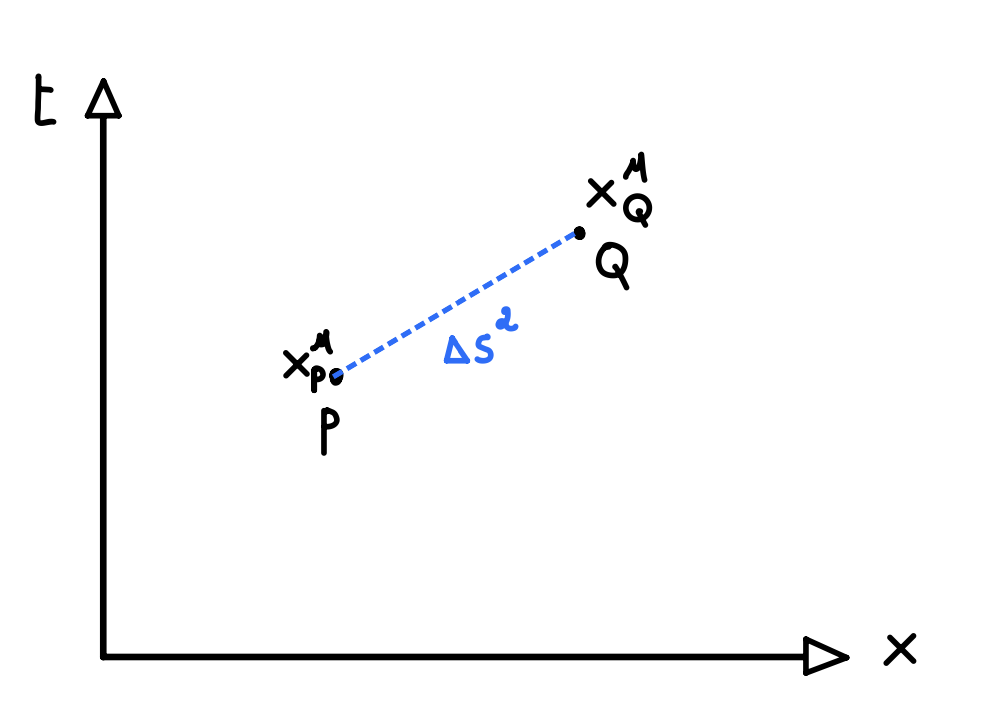
\includegraphics[scale=0.3]{Chapitres/2. Relativité Restreinte/Images/intervalle graph.png}
    \end{center}
    \begin{enumerate}
        \item Supposons qu'un signal lumineux joigne $P$ à $Q$. On a donc $\lt \frac{\Delta \vect{x}}{\Delta t} \rt^2 = v^2 = c^2$. Calculons $(\Delta s )^2$:
        \begin{align}
            (\Delta s )^2  & = -(c\Delta t)^2 + (\Delta \vect{x})^2\\
            \lt\frac{\Delta s}{\Delta t}\rt^2 & = -c^2 + \lt \frac{\Delta \vect{x}}{\Delta t} \rt^2\\
            & =0
        \end{align}
        Ainsi, $\Delta s = 0$. Dans le référentiel $O'$, on aura également $\Delta s' = 0$  car la vitesse de la lumière est la même dans tout les référentiel inertiel.
        \begin{equation}
            \lt \frac{\Delta s'}{\Delta t'} \rt^2 = -c^2 + v'^2 = 0
        \end{equation}
        Il en découle que si l'intervalle s'annule dans un référentiel inertiel, il s'annule dans tout référentiel inertiel. \\
        \item Montrons maintenant que peu importe valeur de $\Delta s$, on a que $\Delta s = \Delta s' $ pour tous référentiels inertiels.

        Comme les deux référentiels sont inertiels, ils sont reliés par une transformation linéaire: 
        \begin{equation}
            x'^{\mu} = \Lambda\indices{^\mu_\alpha} \, x^{\alpha} + a^{\mu}
            \label{def:poincaré}
        \end{equation}
        où $a\in \R^{1,3}$ est un constante et $\Lambda$ une matrice inversible. Les différences sont alors:
        \begin{equation}
            \label{eq:intervalle1}
            \Delta x'^{\mu} = \Lambda\indices{^{\mu}_{\alpha}} \,  \Delta x^{\alpha}
        \end{equation}
        et donc l'intervalle dans les deux référentiels s'écrit : 
        \begin{align}
            \label{eq:intervalle2}
            (\Delta s)^2 & = \eta _{\mu \nu} \, \Delta x^{\mu} \Delta x^{\nu}\\
            \label{eq:intervalle3}
            (\Delta s')^2 & = \eta _{\mu \nu} \, \Delta x'^{\mu} \Delta x'^{\nu}.
        \end{align}
        Autrement dit, $(\Delta s)^2$ et $(\Delta s')^2$ sont des polynômes du second degré en les $\Delta x^{\mu}$, car d'après \ref{def:poincaré}, $x'^\mu$ dépend linéairement de $x^\mu$. On a montré précédemment que si $(\Delta s)^2 = 0$ alors $(\Delta s')^2 = 0$ : les deux polynômes ont donc les mêmes racines. Or, deux polynômes du second degré qui ont les mêmes racines sont proportionnelles, c'est-à-dire qu'il existe $\kappa\in \R$ tel que
        \begin{equation} 
            \label{eq:intervalle4}
            (\Delta s)^2 = \kappa (\Delta s')^2.
        \end{equation}
        L'espace-temps est isotrope, et $\kappa$ ne peut donc que dépendre de la norme de la vitesse relative entre les deux référentiels : $\kappa(\vect{v})=\kappa(\lVert \vect{v} \rVert)$\footnote{Etant une propriété des deux référentiels, $\kappa$ ne peut que dépendre $\vect{v}$. Nous invitons le lecteur à argumenter pourquoi celui-ci ne peut pas dépendre des coordonnées d'espace.}. En particulier, on trouve $\kappa(\Vec{v}) = \kappa(-\vect{v})$. En effectuant le changement de référentiel inverse, on trouve que
        \begin{equation}
            (\Delta s')^2 = \kappa(-\vect{v}) (\Delta s)^2
            \label{eq:intervalle5}
        \end{equation}
        En combinant\ref{eq:intervalle4} avec \ref{eq:intervalle5}, on obtient finalement
        \begin{align}
            (\Delta s)^2 &= \kappa(\vect{v}) \kappa(-\vect{v}) (\Delta s)^2\\
            &= \kappa^2(\Delta s)^2
        \end{align}
        Il vient que $\kappa ^2= 1$ soit $\kappa = \pm 1$. En injectant \ref{eq:intervalle1} dans \ref{eq:intervalle3}, puis en utilisant la relation \ref{eq:intervalle4}, on trouve que
        \begin{equation}
            \eta_{\mu\nu} \, \Delta x^\mu \Delta x^\nu = \kappa \, \eta_{\alpha\beta} \, \Lambda\indices{^\alpha_{\mu}} \, \Lambda\indices{^\beta_{\nu}}\, \Delta x^\mu \Delta x^\nu
        \end{equation}
        soit (en notation matricielle) :
        \begin{equation}
            \label{eq:Lorentz pre}
            \eta = \kappa \,\eta'=\kappa \,\Lambda^T\eta \Lambda
        \end{equation}
        Comme $\eta$ est une forme quadratique symétrique et $\eta'$ est un changement de base de $\eta$ ($\Lambda$ est inversible), le \textit{théorème de Sylvester}\footnote{c.f. votre cours d'algèbre de BA1.} impose que la signature de $\eta'$ ne change pas, et donc que $\kappa=1$. On peut ainsi conclure que $(\Delta s')^2 = (\Delta s)^2$.
    \end{enumerate}
\end{proof}

\section{Transformations de Lorentz et de Poincaré}

On définit les transformations de Poincaré comme l'ensemble des isométries sur l'espace-temps munie de la (pseudo-)métrique de Minkowski $(\R^{1,3},s)$, c'est-à-dire les transformations qui relient des référentiels inertiels et telles que la vitesse de la lumière $c$ soit conservée.

Soient deux référentiels inertiels $O$ et $O'$ qui ont respectivement comme coordonnées $x^{\alpha}$ et $x^{\alpha '}$. 
Comme les deux référentiels sont inertiels ils doivent être reliés par la transformation \ref{def:poincaré}. 

Comme vu dans la section précédente, en prenant $\kappa = 1$ dans la relation \ref{eq:Lorentz pre}, on trouve que

\begin{equation}
    \label{eq:Lorentz}
    \boxed{\Lambda ^{T} \eta \Lambda = \eta}
\end{equation}

L'ensemble des matrices satisfaisant à l'équation \ref{eq:Lorentz} est appelé le \textit{groupe de Lorentz} O$(3,1)$. L'ensemble des couples $(\Lambda,a)$ satisfaisant à \ref{eq:intervalle1} et donc à \ref{eq:Lorentz} est appelé \textit{groupe de Lorentz inhomogène} ou le \textit{groupe de Poincaré} $IO(3,1)$. 

\begin{rmk}
Lorsque $\eta = \text{diag}(-1,...,-1,1,...,1)$ avec $p$ fois -1 et $q$ fois +1, on appelle le groupe vérifiant \ref{eq:Lorentz} IO$(p,q)$
    
\end{rmk}
\begin{rmk}
    Dans le cas particulier $p =0$ et $q=3$, on a le groupe IO(3) c'est-à-dire avec $\Lambda ^{T} \Lambda = I_{3x3}$. 
\end{rmk}

Les transformations telles que $\Lambda =  I$ appartiennent au groupe de translation.

\subsection{Groupe de Lorentz}

Le groupe de Lorentz O(3,1) possède deux sous-groupes non-triviaux. En particulier, il possède quatre composantes non-connexes.

\begin{enumerate}
    \item En reprenant la relation $\Lambda ^{T} \eta \Lambda = \eta$, et calculant le déterminant:
    \begin{equation}
        \det \Lambda^{T} \det \eta \det\Lambda = \det \eta \\
        \implies \det\Lambda = \pm 1
    \end{equation}
    Comme il est impossible de passer continûment d'un élément de $\det =1$ à un élément de $\det = -1$, le groupe possède deux composantes non-connexes. On note O$(3,1)_\pm$ la partie du groupe de Lorentz à $\det = \pm 1$.\\
    Uniquement la composante O(3,1)$_+$ est un sous-groupe de O(3,1), appelé le groupe spécial de Lorentz noté SO(3,1)\footnote{En effet, c'est la seule des deux composantes qui inclut l'élément identité.}. \\

    \item Réécrivons la relation de définition \ref{eq:Lorentz} du groupe de Lorentz. En composantes, on trouve
    \begin{equation}
        \eta_{\alpha \beta}\, \Lambda\indices{^\alpha_{\mu}} \,\Lambda\indices{^\beta_{\nu}} = \eta_{\mu \nu}
    \end{equation}
    Ainsi, pour la composante $\mu = \nu =0$:
    \begin{align}
        \eta_{0 0} &= \eta_{\alpha \beta} \,\Lambda\indices{^\alpha_{0}} \, \Lambda\indices{^\beta_{0}} \\
        -1 &= -(\Lambda\indices{^0_{0}})^2 + \sum_{k}(\Lambda\indices{^k_0})^2\\
        (\Lambda\indices{^0_0})^2 &= 1 + \sum_{k}(\Lambda\indices{^k_0})^2\\
        \implies (\Lambda\indices{^0_0})^2 &\geq 1
    \end{align}
    On trouve donc de nouveau deux composantes non-connexes notées O(3,1)$^\uparrow$ (si $\Lambda\indices{^0_0} \geq 1$) et O(3,1)$^\downarrow$ (si $\Lambda\indices{^0_0} \leq - 1$). Uniquement O(3,1)$^\uparrow$ est un sous-groupe de O(3,1), appelé le sous-groupe orthochrone de Lorentz.
\end{enumerate}
Le groupe O(3,1)$^\uparrow_+ \equiv$ SO(3,1)$^\uparrow$ est un sous-groupe normal de O(3,1), et pour simplifier le langage, nous l'appelerons également le groupe de Lorentz\footnote{Les transformations qui inversent l'orientation de l'espace ou du temps ne nous intéressent que rarement.} Nous renvoyons vers votre cours de théorie des groupes pour une étude détaillée du groupe de Lorentz.
\subsection{Rappel : les transformations de Lorentz}

\begin{exmp}
    Une rotation autour de l'axe $z$ peut être décrite par la matrice
    \begin{equation}
        \Lambda = \begin{pmatrix}
1 & 0 & 0 & 0\\
0 & \cos{\theta} & \sin{\theta} & 0\\
0 & -\sin{\theta} & \cos{\theta} & 0\\
0 & 0 & 0 & 1\\
\end{pmatrix}
    \end{equation}
    En notant $\vect{x}'=\Lambda \vect{x}$, on peut réécrire cette transformation comme
    \begin{align}
    \left\{
\begin{array}{l}
  t' =t \\
  x' = x\cos{\theta} + y\sin{\theta}\\
  y' = -x\sin{\theta} + y\cos{\theta}\\
  z' = z
\end{array}
\right.
\end{align}
Correspondant bien à une rotation autour de $z$.
\end{exmp}

\begin{exmp}
    Un \textit{boost} dans la direction $x$ peut être décrite par la matrice
    \begin{equation}
        \Lambda = \begin{pmatrix}
\cosh{\phi}& -\sinh{\phi} & 0 & 0\\
-\sinh{\phi} & \cosh{\phi} & 0 & 0\\
0 & 0 & 1 & 0\\
0 & 0 & 0 & 1\\
\end{pmatrix}
    \end{equation}
    De nouveau, on peut réécrire cette transformation comme 
\begin{align}
\label{eq:4.2.1}
    \left\{
\begin{array}{l}
  t' = t\cosh{\phi} - x\sinh{\phi} \\
  x' = -t\sinh{\phi} + x\cosh{\phi}\\
  y' = y\\
  z' = z
\end{array}
\right.
\end{align}
\end{exmp}
Pour montrer que cette transformation correspond bien à un boost dans la direction $x$, nous allons effectuer un changement de variable qui nous ramène aux transformations de Lorentz sous leur forme usuelle.

Posons $-1 < v\deq\tanh\phi < 1$ . Définissons de plus $\gamma \deq \cosh\phi$. Alors, $\sinh\phi = v \gamma$ et la transformation \ref{eq:4.2.1} se réécris comme
\begin{align}
\left\{
\begin{array}{l}
  t' = \gamma(t - vx) \\
  x' = \gamma(x - vt)\\
  y' = y \\
  z' = z
\end{array}
\right.
\end{align}
On peut également déduire l'expression de $\gamma$ en fonction de $v$ :
\begin{align}
    \cosh^2{\phi} - \sinh^2{\phi} = 1\\
    \implies  1 - \tanh^2{\phi} = \frac{1}{\cosh^2{\phi}}
\intertext{Alors, par leur définition :}
    1 - v^2 = \frac{1}{\cosh^2{\phi}}
\intertext{Soit}
    \gamma = \sqrt{\frac{1}{1-v^2}}
\end{align}

\section{Structure causale de l'espace-temps de Minkowski}

\subsection{Le cône de lumière}
\vspace{5pt}
\begin{theoremframe}
    \begin{defi}
        Le \textit{cône de lumière} de $P \in \R^{1,3}$ noté $C_P$ est l'ensemble des points à distance nulle de $P$.
        \begin{equation}
            C_P = \ltc Q \in \R^{1,3} \mid \Delta s_{PQ} = 0\rtc
        \end{equation}

    \end{defi}
\end{theoremframe}
On se rappelle que l'intervalle d'espace-temps peut se réécrire comme:
\begin{equation}
    (\Delta s)^2 = -(\Delta t)^2 + \sum_{i}(\Delta x^{i})^2
\end{equation}
La condition $(\Delta s)^2 = 0$ implique donc que $\Delta t =
\sqrt{(\Delta x)^2 + (\Delta y)^2 + (\Delta z)^2}$, qui est la contrainte d'un 4-cône (à tout temps $\Delta t$ fixe, il s'agit d'une sphère de rayon $\Delta t$).

\begin{theoremframe}
    \begin{notat}
        Le cône de lumière va diviser l'espace de Minkowski en 3 régions tel que:
        \begin{enumerate}[label = \roman*.]
            \item \textit{Le futur absolu} de $P$ correspond au cône de lumière supérieur rempli noté $C_{P}^{+}$.
            \item \textit{Le passé absolu} de $P$ correspond au cône de lumière inférieur rempli noté $C_{P}^{-}$. 
            \item \textit{L'ailleurs absolu} de $P$ correspond au complémentaire de $C_P^\pm $.
        \end{enumerate}
    \end{notat}
\end{theoremframe}
Ces trois régions sont illustrés sur la figure \ref{fig:2.1}. Justifions cette terminologie : soient $P,Q\in \R^{1,3}$.

\begin{theoremframe}
    \begin{propri}
         Si $Q \in C_P^+$ (resp. $C_P^-$), alors $Q$ se produit après (resp. avant) $P$ pour tout référentiel inertiel.
    \end{propri}
\end{theoremframe}
\begin{proof}
    Voir séances d'exercices.
\end{proof}
La causalité est fondamentale dans une théorie physique. La propriété précédente assure que la causalité de deux évènements causalement connectés (ils se trouvent dans le cône de lumière de l'autre) est conservée pour tout référentiel inertiel. 
    \begin{figure}[H]
     \centering
        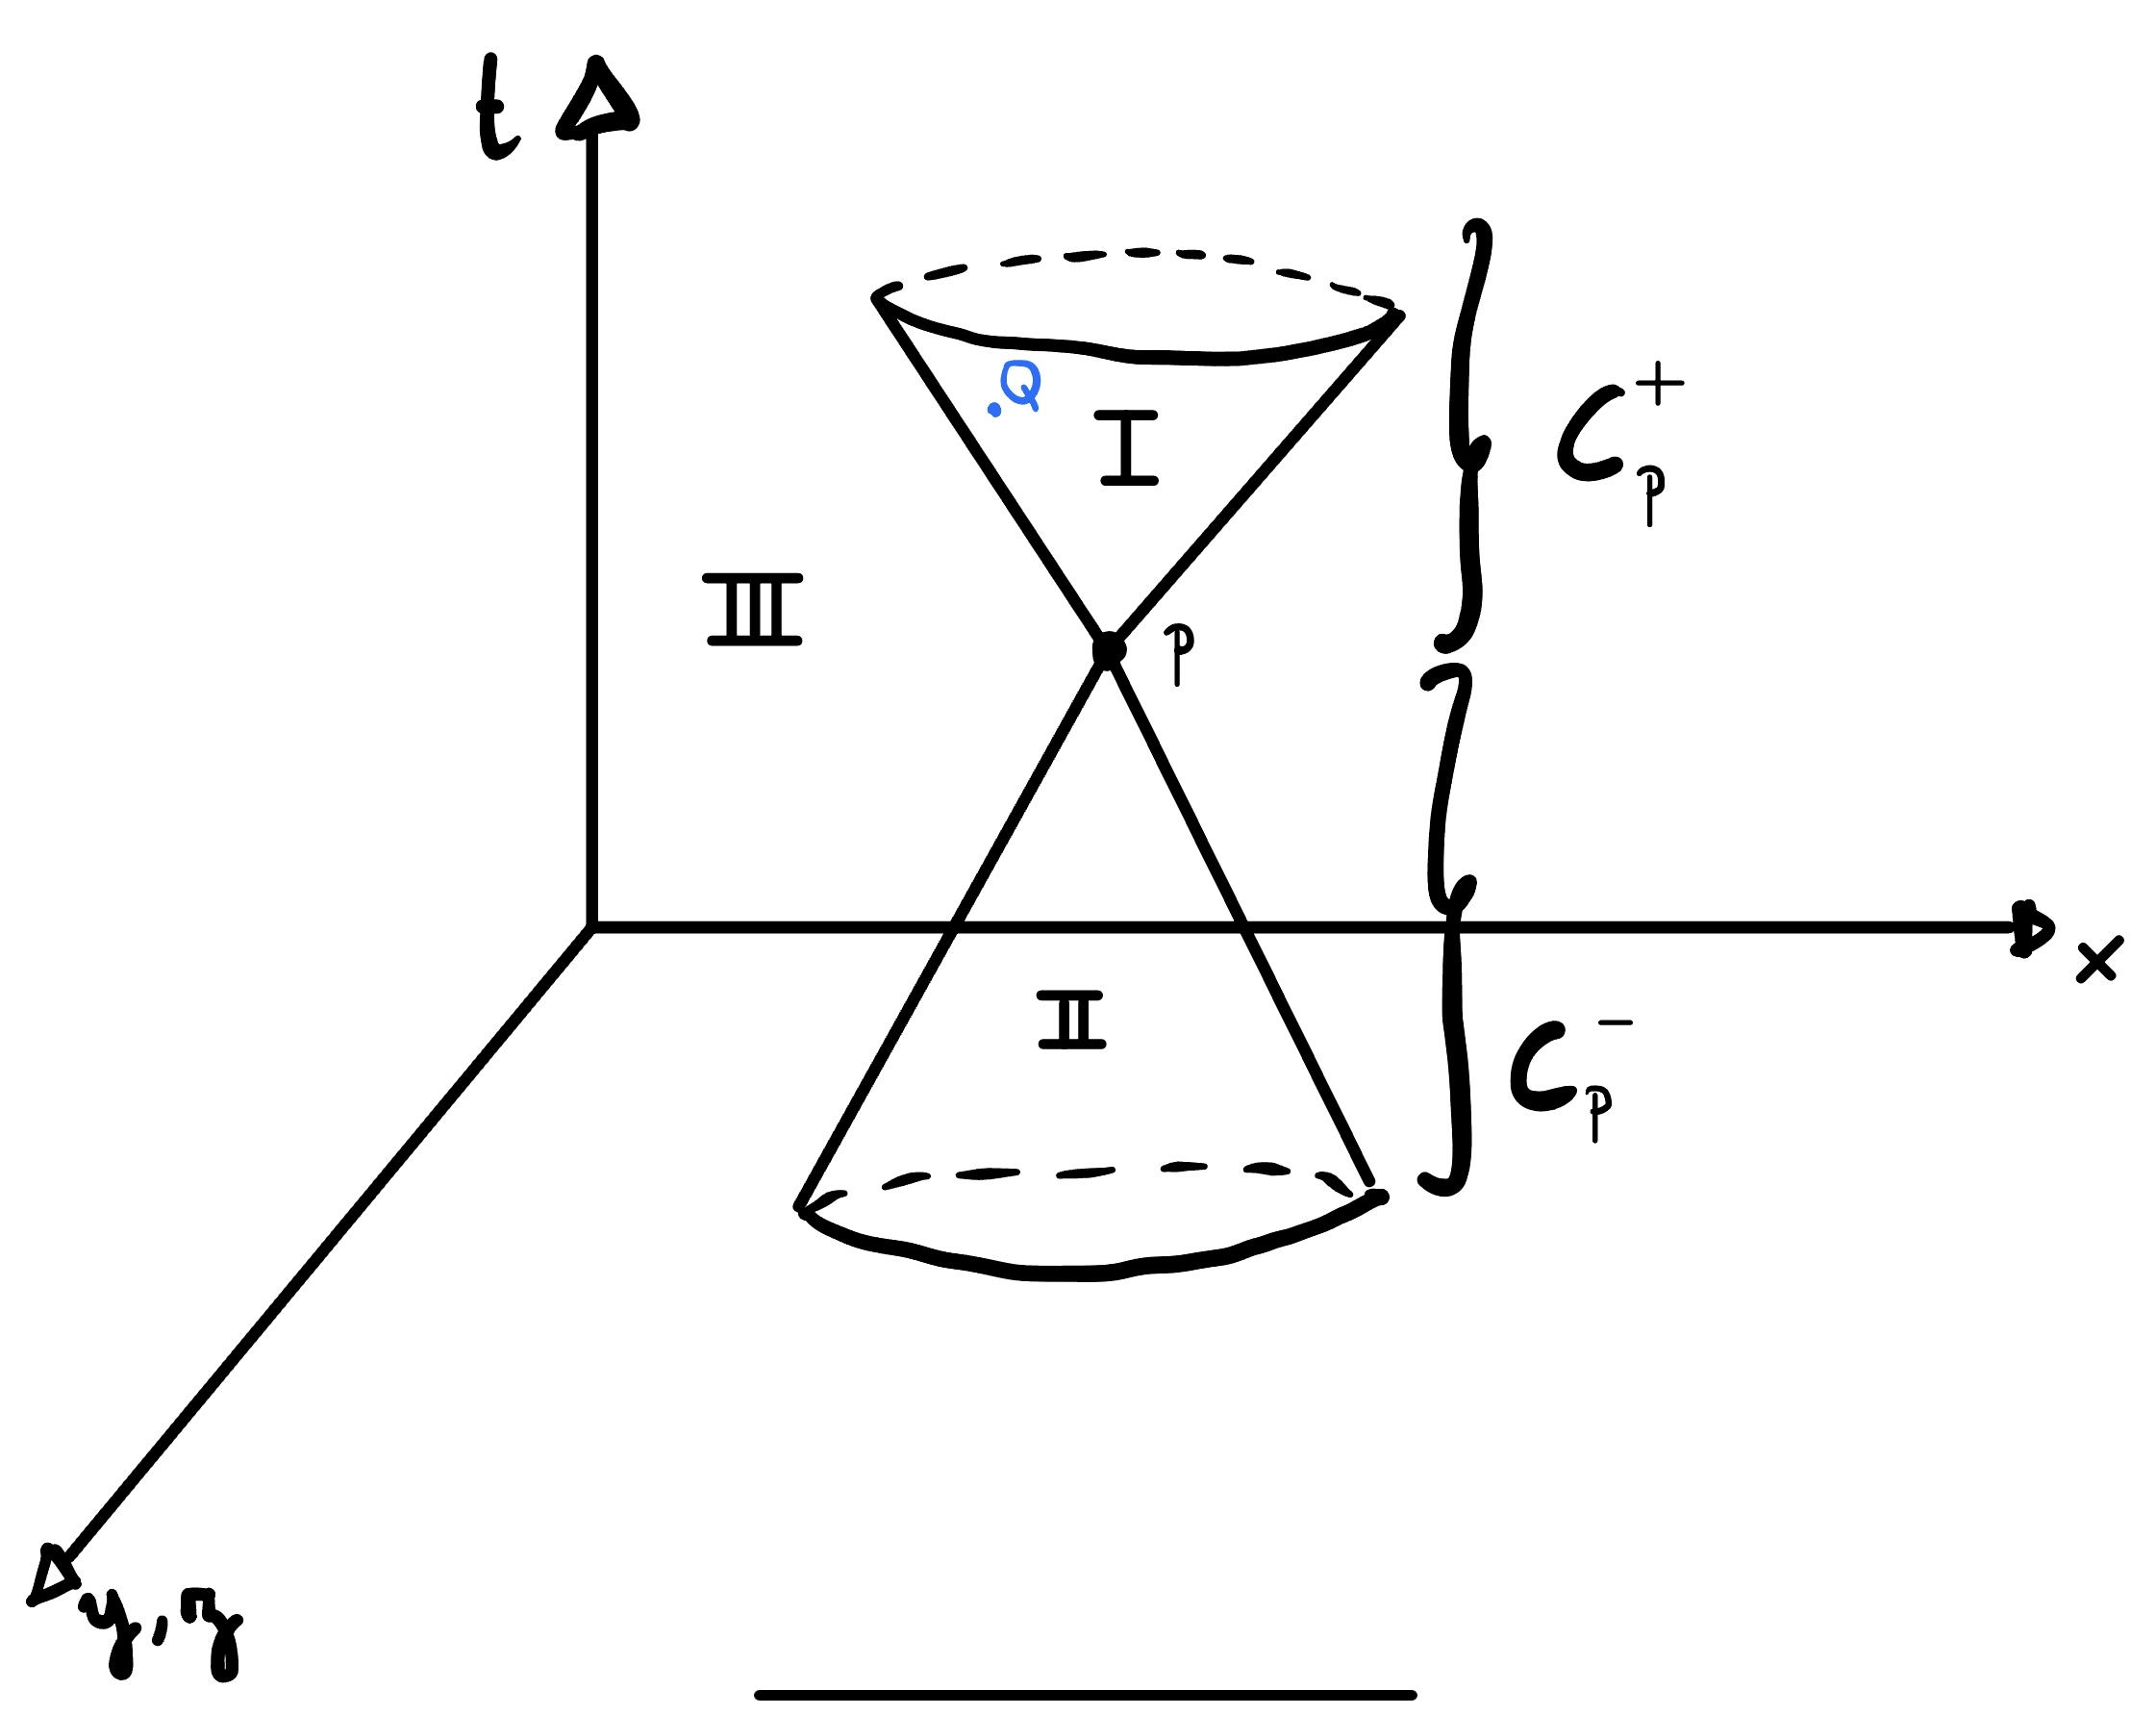
\includegraphics[width=0.5\textwidth]{Chapitres/2. Relativité Restreinte/Images/Cone de lumière avec point Q dans 1.jpg}
        \caption{Le cône de lumière de $P$ représenté dans l'espace $\R^{1,2}$}
        \label{fig:2.1}
\end{figure}

\begin{theoremframe}
    \begin{propri}
        Si $(\Delta s_{PQ})^2 < 0$ alors on peut trouver un référentiel inertiel pour lequel $P$ et $Q$ se passent au même endroit c'est-à-dire que $\Delta x^{i}_{PQ }= 0$.
    \end{propri}
\end{theoremframe}
\begin{proof}
    Voir séances d'exercices.
\end{proof}
    Comme on est dans le cas où $(\Delta s_{PQ})^2 < 0$ (intérieur du cône), $P$ et $Q$ sont en contact causal. Graphiquement, la propriété précédente est facile à démontrer, comme le montre la figure \ref{fig:2.2}. En effet, comme $Q$ se trouve à l'intérieur du cône de lumière de $P$, et en se rappelant de l'effet d'un boost sur les axes du nouveau référentiel $O'$, il est possible de trouver un référentiel dont l'axe de temps $t'$ relie $P$ à $Q$. Ainsi, $\Delta x = 0$. Il est en revanche impossible de trouver un référentiel inertiel dans lequel les deux évènements ont lieu en même temps.
\begin{figure}[H]
    \begin{center}
        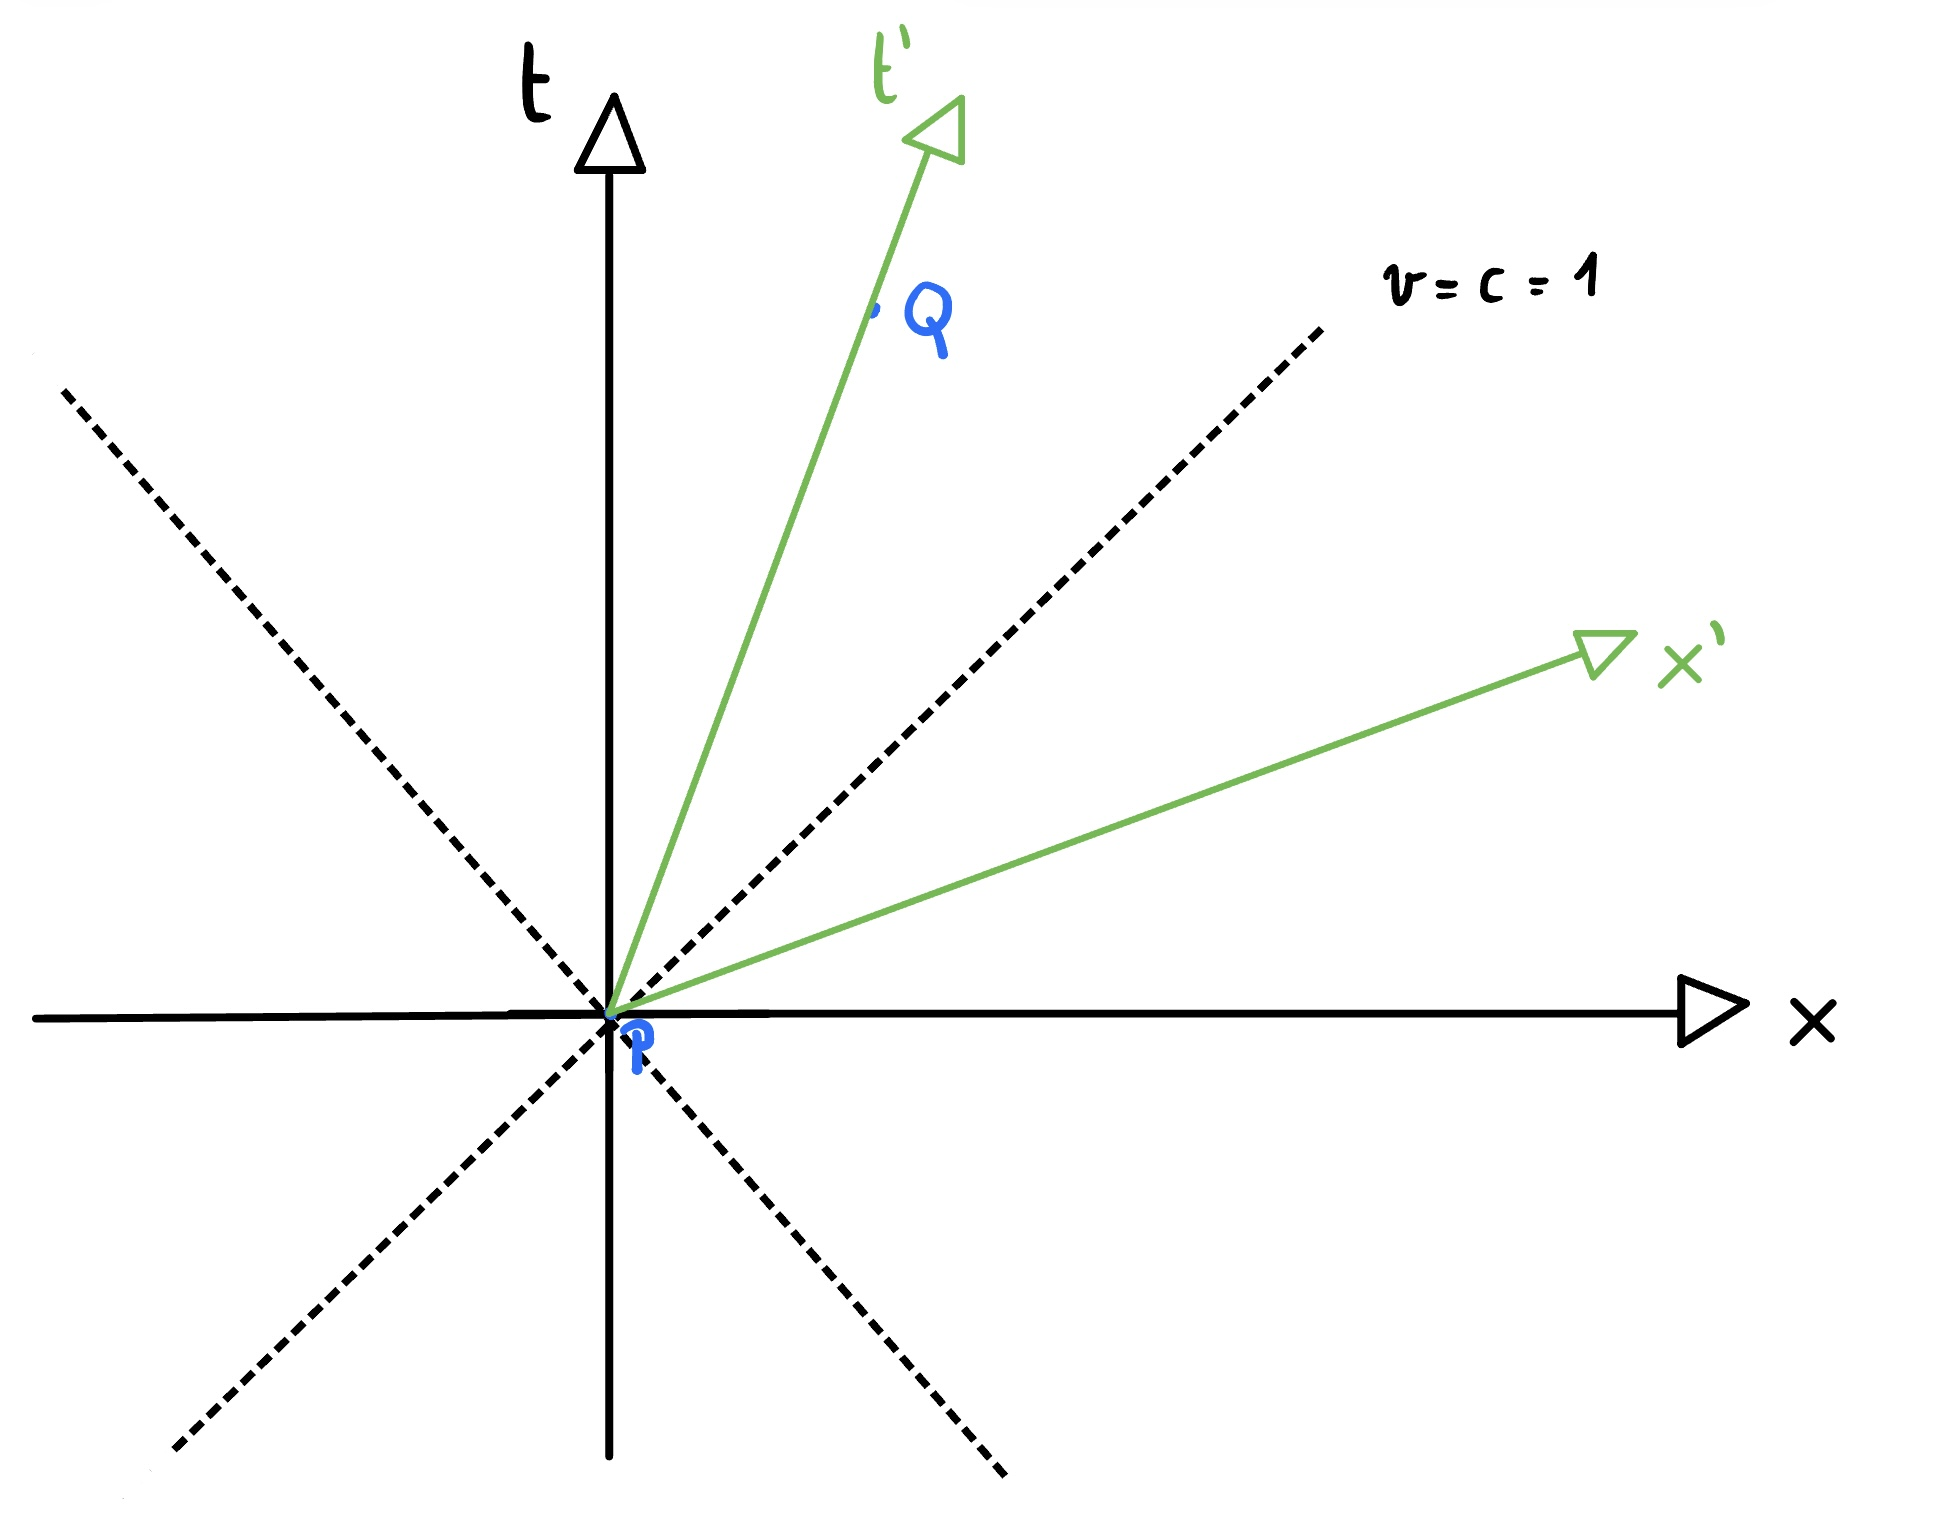
\includegraphics[scale=0.1]{Chapitres/2. Relativité Restreinte/Images/Changement de variable.jpg}
        \caption{Il existe un référentiel tel que deux points causalements connectés se passent au même endroit.}
        \label{fig:2.2}
    \end{center}
\end{figure}
\quad\\
\\

\begin{theoremframe}
    \begin{propri}
        Si $Q$ appartient à l'ailleurs absolu de $P$, alors :
        \begin{enumerate}[label = \roman*.]
            \item Il n'existe pas de référentiel inertiel tel que $Q$ se passe au même endroit que $P$.
            \item Il existe des référentiels inertiels tels que $Q$ se passe avant, en même temps ou après $P$.
        \end{enumerate}
    \end{propri}
\end{theoremframe}
\begin{proof}
    Voir séances d'exercices.
\end{proof}

    Comme $Q$ n'est pas dans le cône de lumière, $P$ et $Q$ ne peuvent pas être en contact causal. On peut effectuer un boost tel que deux événements $P$ et $Q$ ont lieu en même temps ( c'est-à-dire que $\Delta t' = 0$). 

    Les cônes de lumière donnent à l'espace-temps de Minkowski une structure très différente de l'espace-temps euclidien usuel de la théorie de Newton. Dans cette dernière, il n'y a pas de transformation mélangeant espace et temps , et il existe une division logique de l'espace-temps en "tranches", représentant tout l'espace à un temps donné. En particulier:
    \begin{enumerate}
        \item la notation de simultanéité est absolue (non-ambiguë).
        \item les trajectoires d'une particule sont contraintes uniquement par $\Delta t> 0$; On peut avoir $v>c$.
    \end{enumerate}
    En relativité restreinte, la notion de simultanéité devient relative au référentiel choisi et d'autre part, l'espace-temps est structuré par les cônes de lumières en tout point qui déterminent les trajectoires possibles des particules (structure causale). Par l'invariance de $c$ pour tout référentiel inertiel, on peut déduire que les cônes de lumières sont les mêmes pour tout référentiel inertiel.
    \begin{figure}[H]
        \centering
        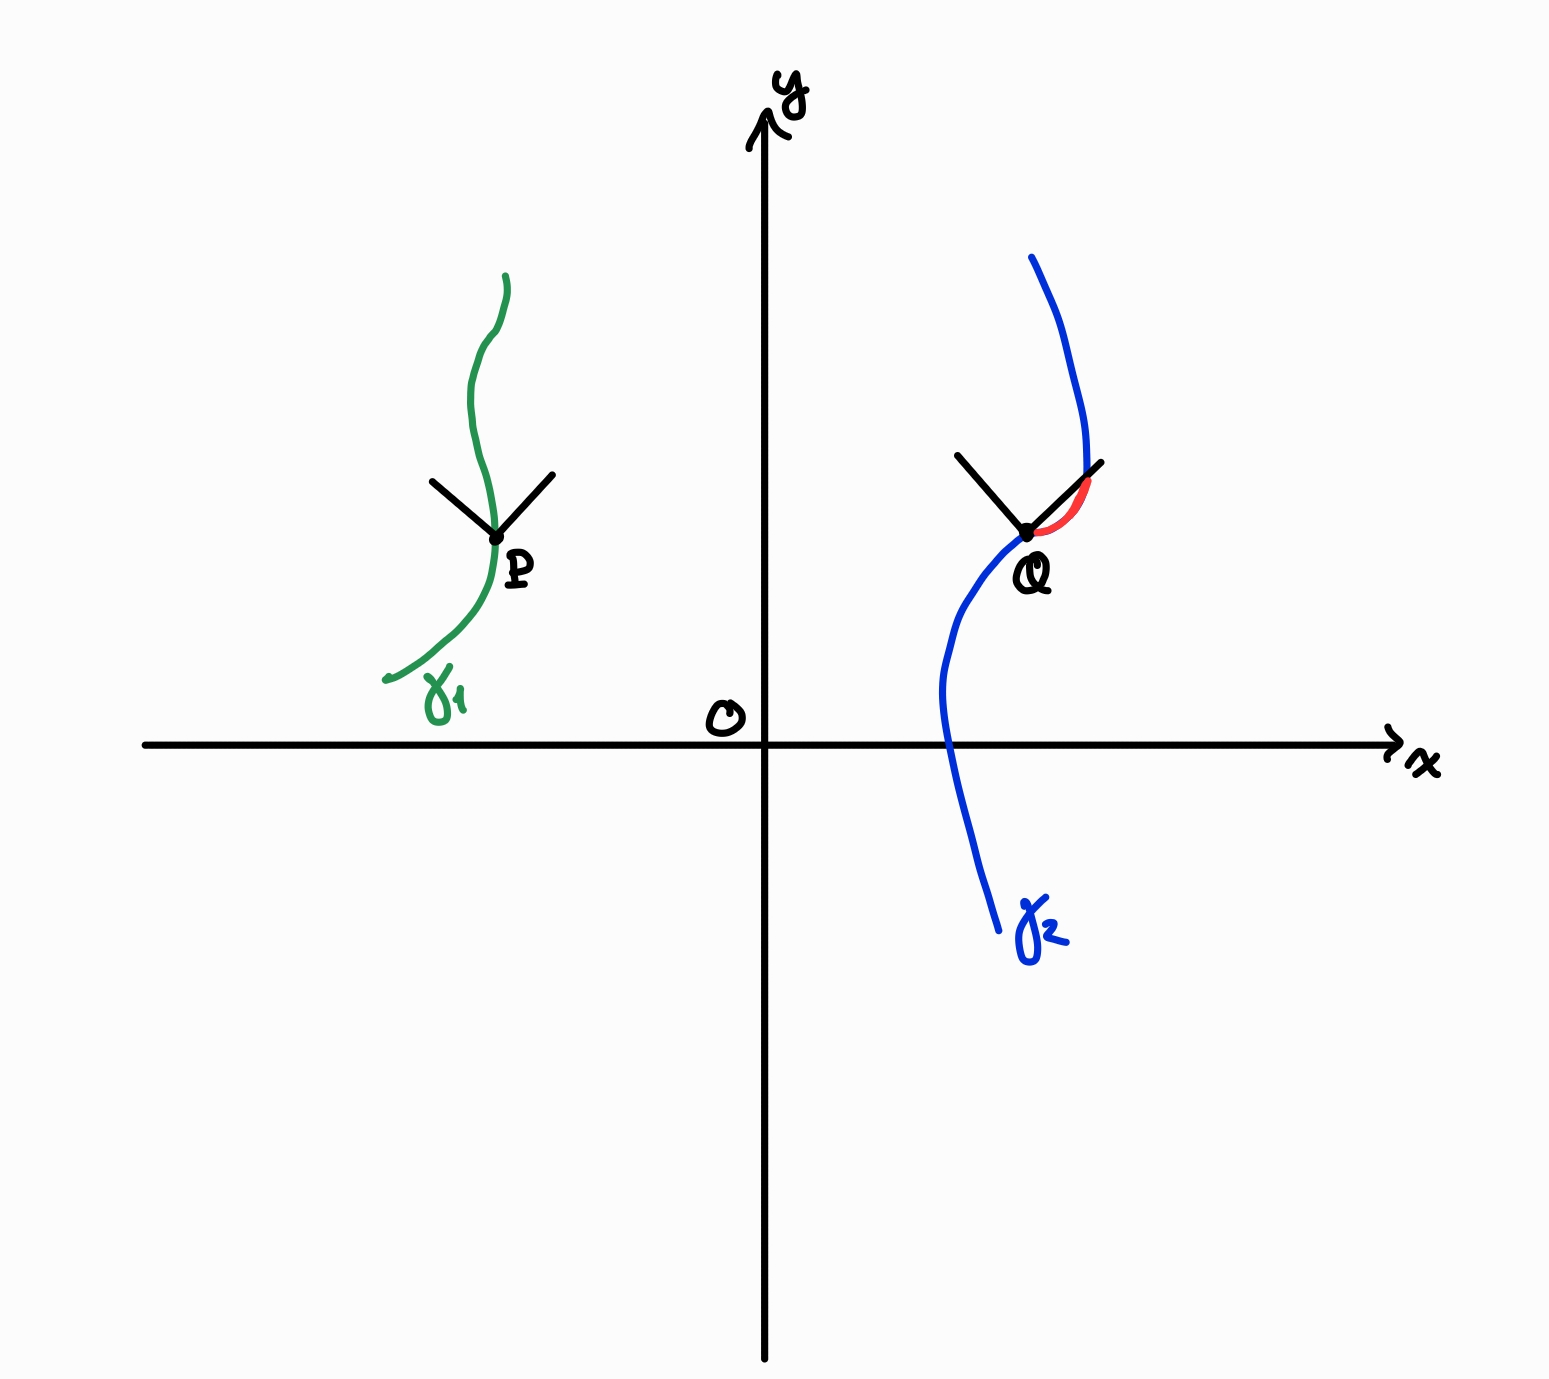
\includegraphics[width=0.5\linewidth]{Chapitres/2. Relativité Restreinte/Images/Courbes non causales.png}
        \caption{En $\R^{1,3}$, uniquement les trajectoires du type $\gamma_1$ sont admissibles. La courbe $\gamma_2$ ne peut pas représenter la trajectoire d'une particule car son tracé n'est plus contenu dans le cône de lumière de $Q$.}
        \label{fig:2.3}
    \end{figure}
\subsection{Temps propre}

Soient deux évènements $P$ et $Q$ causalement liés. 
\begin{theoremframe}
    \begin{defi}
        Le temps propre séparant $P$ et $Q$ est défini comme:
        \begin{equation}
            (\Delta s_{PQ})^2 = -(\Delta \tau)^2
        \end{equation}
    \end{defi}
\end{theoremframe}

Si $P$ et $Q$ représentent une particule ponctuelle à des temps différents, le temps propre $\Delta \tau $ est le temps écoulé entre deux évènements pour un observateur attaché au mouvement. En effet, comme les évènements sont causalement liés, il existe un référentiel dans lequel $P$ et $Q$ se passent au même endroit, et donc $(\Delta s)^2=-(\Delta t')^2 =$ et donc $\Delta t' = \Delta \tau$ dans ce référentiel.

\subsection{Courbes causales}
\vspace{5pt}
\begin{theoremframe}
    \begin{rap}
        Soit un ouvert $I \in \R$. Une application lisse
        \begin{align}
            \gamma :\, I &\longrightarrow \R^{1,3}\\ \lambda &\longmapsto \gamma(\lambda)
        \end{align}
         est appelée courbe (lisse) sur $\R^{1,3}$. Nous noterons explicitement les coordonnées de la courbe $\gamma(\lambda) = x^\mu (\lambda)$.
    \end{rap}
\end{theoremframe}
\begin{theoremframe}
    \begin{propri}
        Le champ de vecteurs tangent à la courbe $v$ est défini par
        \begin{equation}
            v^\mu = \frac{\td x^\mu}{\td \lambda}
        \end{equation}
    \end{propri}
\end{theoremframe}
La courbe est dite de genre $\left\{
\begin{array}{l}
 \text{temps} \\
 \text{espace}\\
 \text{lumière}
\end{array}
\right.$ en un point
si la norme du champ tangent $ v^2 = v_{\alpha}v^{\alpha}$ est
$\left\{
\begin{array}{l}
 < 0 \\
 > 0\\
 = 0
\end{array}
\right.$ en ce point. Notons que la notation en $v^\alpha$ du champ tangent sera réservé aux courbes paramétrisées par leur temps propre $\tau$ (pour des courbes de type temps).
\begin{exmp}
    La norme du vecteur $v = (1,0,0,0)$ est donnée par 
    \begin{equation}
        \eta_{\alpha \beta}\,v^{\alpha} v^{\beta} = (-1)\, v^{0} v^{0} =-1
    \end{equation}
    et n'est donc pas définie positive, contrairement au cas euclidien.
\end{exmp}
\begin{theoremframe}
    \begin{defi}
        Une courbe est dite \emph{causale} si en tout point de la courbe, son vecteur tangent est
        \begin{enumerate}[label = \roman*.]
            \item de genre temps ou lumière.
            \item orienté vers le futur ($\frac{\td x^0}{\td\lambda}>0$).
        \end{enumerate}
    \end{defi}
\end{theoremframe}
\subsection{Longueur Minkowski d'une courbe causale}

D'après la définition du temps propre de deux évènements causalement liés
\begin{equation}
    \label{eq:temps propre}
   (\Delta \tau)^{2} = -(\Delta s)^2 = (\Delta t)^2 - \sum_{i}(\Delta x^{i})^2 
\end{equation}

on définit le temps propre infinitésimal
\begin{equation}
    \td\tau ^2 = -\td s^{2} = \td t^2 - \sum_{i} (\td x^{i})^2
\end{equation}
\begin{figure}
    \centering
    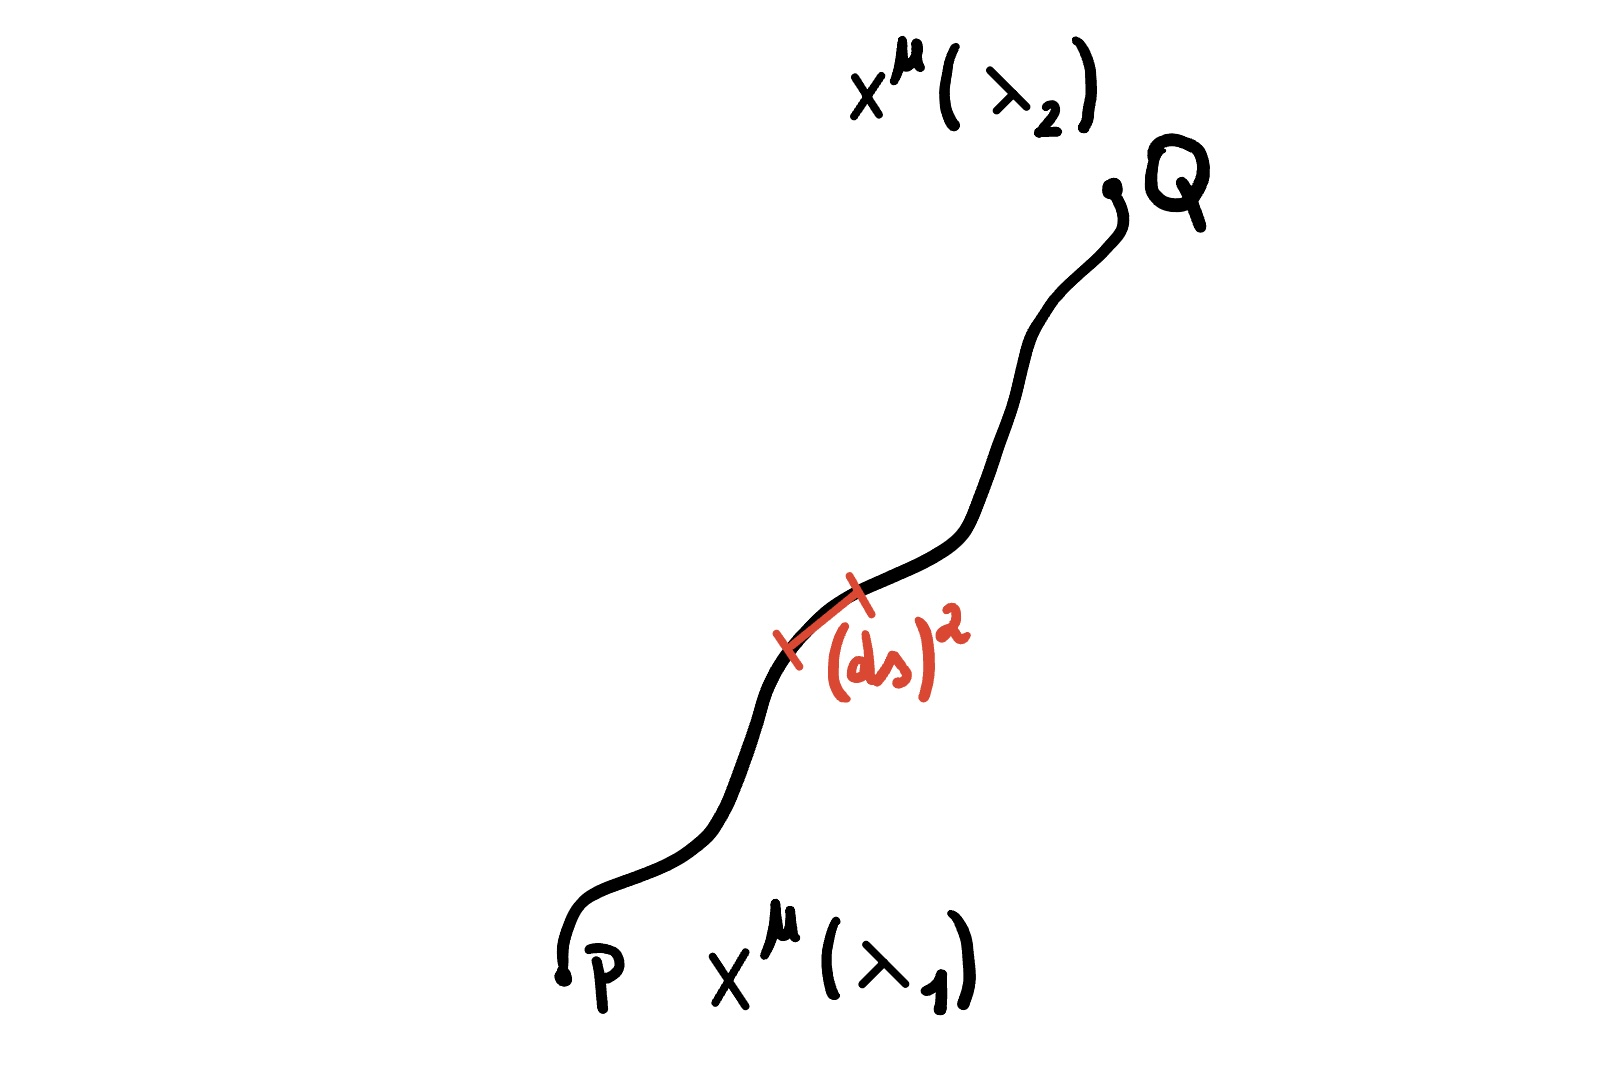
\includegraphics[width=0.5\linewidth]{Chapitres/2. Relativité Restreinte/Images/Coubre.jpg}
    \caption{}
    \label{fig:2.4}
\end{figure}
Cette définition permet nous permet de définir le temps propre d'une courbe causale $\gamma$ arbitraire comme
\begin{align}
    \tau_\gamma &= \int_{\gamma} \td\tau\\
    &= \int^{\lambda_{2}}_{\lambda_{1}}\left(\frac{\td\tau}{\td\lambda}\right)\td\lambda\\
    &= \int^{\lambda_{2}}_{\lambda_{1}} \td \lambda \, \sqrt{\left(\frac{\td t}{\td\lambda}\right)^2 - \sum_{i}\left(\frac{\td x^{i}}{\td\lambda}\right)^2} 
\end{align}
Et est le temps mesuré par un observateur suivant la trajectoire. 
\begin{theoremframe}
    \begin{propri}
        Le temps propre entre deux événements causalement reliés défini par \ref{eq:temps propre} correspond au temps propre de la droite reliant les deux évènements. De plus, la courbe qui maximise le temps propre entre deux évènements est la droite.
    \end{propri}
\end{theoremframe}
\begin{proof}
    Voir séances d'exercices.
\end{proof}
En effet, le temps propre de deux courbes causales distinctes reliant deux événements n'est en général pas identique. Un exemple de cette propriété est le "paradoxe" des jumeaux.

\begin{exmp}[Paradoxe des jumeaux\footnote{Disclaimer: il s'agit d'une expérience de pensée. Aucune fusée n'a été blessée au cours de cette expérience.}]
    Supposons que deux jumeaux sur Terre possèdent chacun une horloge atomique qui affiche la même heure. Posons leur genre = M. L'un des jumeaux est envoyé dans l'espace à une vitesse proche de celle de la lumière avec cette horloge. Quand il revient sur Terre, en comparant les deux horloges, le jumeaux étant resté sur terre est plus jeune que celui parti dans l'espace. 
\end{exmp}
Pour expliquer ce "paradoxe" (ce n'en est pas réellement un\footnote{\href{https://www.youtube.com/watch?v=ppX7Qjbe6BM}{Vidéo intéressante sur le sujet}.}), intéressons-nous à la situation simplifiée suivante, où un jumeau passe directement de $A$ à $C$, et l'autre jumeau fait un détour par $B'$.
\begin{figure}[H]
    \centering
    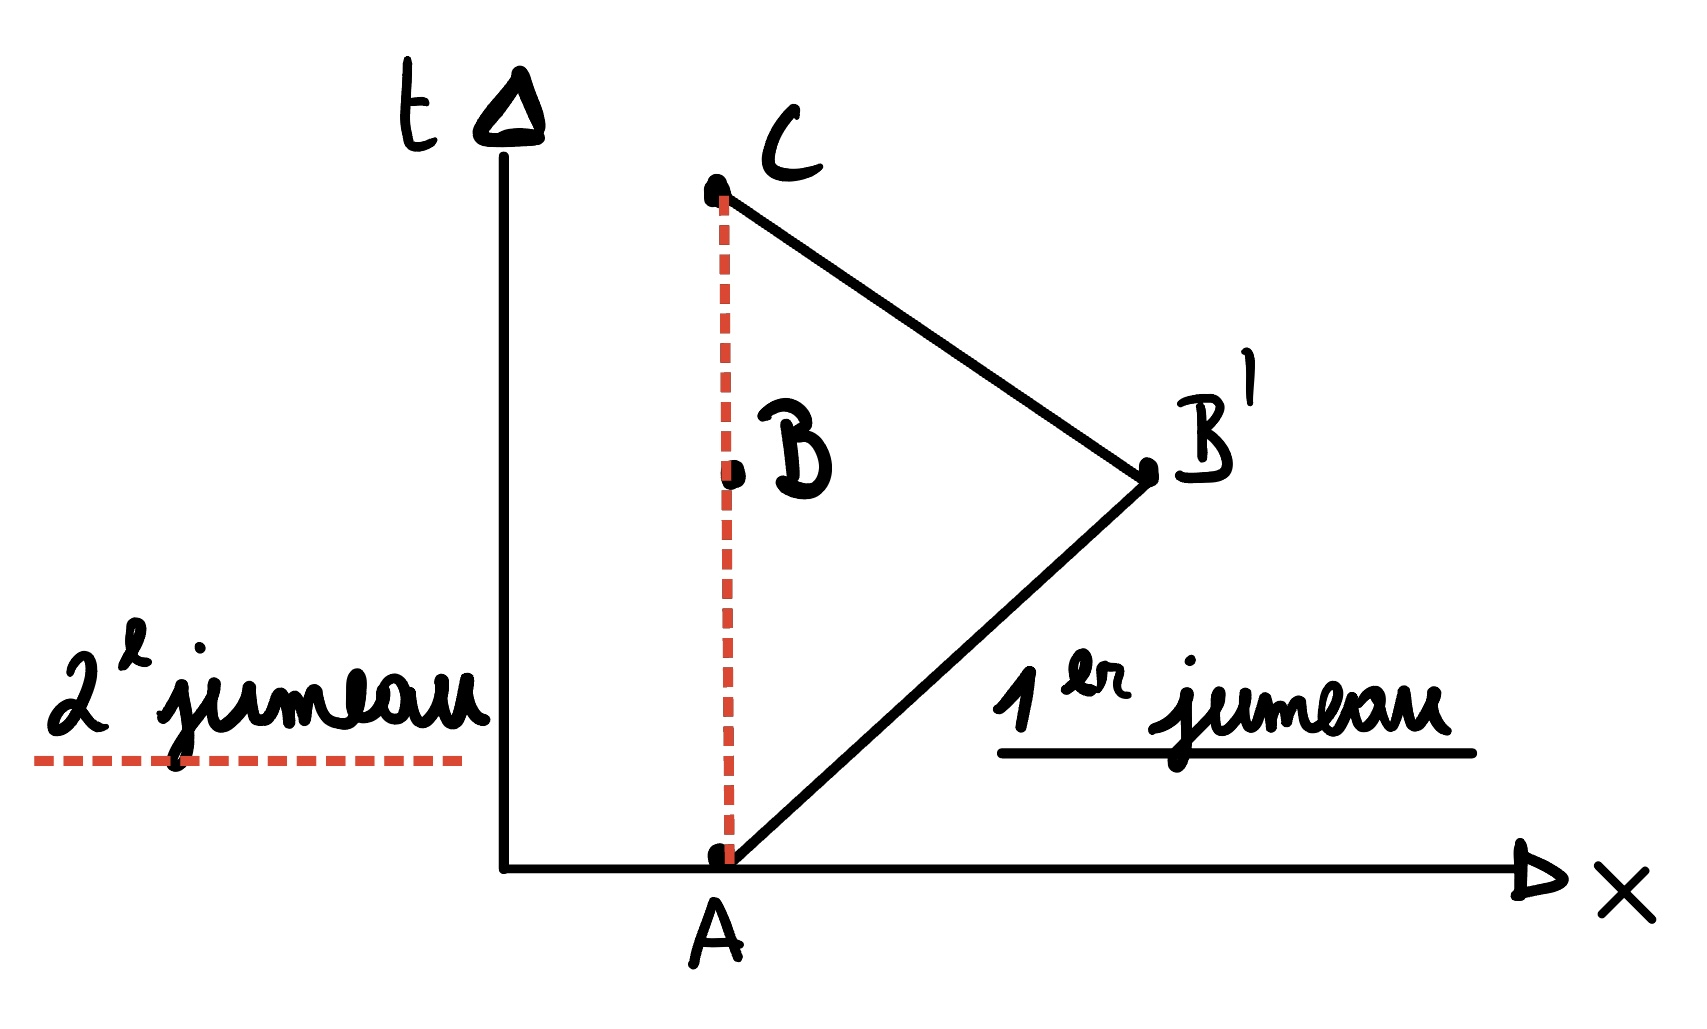
\includegraphics[width=0.5\linewidth]{Chapitres/2. Relativité Restreinte/Images/Deux jumeaux.jpg}
    \caption{}
    \label{fig:2.5}
\end{figure}

Calculons le temps propre des deux chemins. Dans le référentiel $O$, on a pour le deuxième jumeau
\begin{equation}
    (\Delta \tau_{ABC})^2 = (\Delta t)^2
\end{equation} 
Pour le premier jumeau, comme $B'=(\frac{\Delta t}{2},\Delta x)$, on trouve
\begin{align}
        (\Delta \tau_{AB'C})^2 &= (\Delta \tau_{AB'} + \Delta \tau_{B'C})^2\\
        &= 4(\Delta \tau_{AB'})\\
        &= 4 \left(\left(\frac{\Delta t}{2}\right)^2 - (\Delta x)^2\right)\\
        &= 4 \left(\left(\frac{\Delta t^2}{4}\right) - (\Delta x)^2\right)
    \end{align}
    On peut définir (graphiquement) $v = \dfrac{\Delta x}{(\Delta t/2)} = \dfrac{2 \Delta x}{\Delta t}$ qui est tel que $v^2 = \frac{4(\Delta x)^2}{(\Delta t)^2}$ et donc
    \begin{align*}
        (\Delta \tau_{AB'C})^2 &= (\Delta t)^2(1 - v^2)\\
        &< (\Delta t)^2
    \end{align*}

Le temps propre du premier jumeaux (voyageur) est plus petit que le temps propres du jumeau 2 (au repos). 
\begin{center}
    \textit{Le temps s'écoule plus lentement quand on est en mouvement.}
\end{center}

\subsection{Horizon des événements} 

Soit $\mathcal{S} \subset \R^{1,3}$  un sous-ensemble de Minkowski. 
\begin{theoremframe}
    \begin{defi}
        Le \emph{futur chronologique} $I^{+}(\mathcal{S})$ est l'ensemble des points de $\R^{1,3}$ qui sont reliés à un point de $\mathcal{S}$ par une courbe causale de genre temps. 
    \end{defi}
\end{theoremframe}
\begin{theoremframe}
    \begin{defi}
        Le \emph{futur causal} $J^{+}(\mathcal{S})$ est l'union de $\mathcal{S}$ avec tous les points de $\R^{1,3}$ qui sont reliés à un point de $\mathcal{S}$ par une courbe causale. 
    \end{defi}
\end{theoremframe}

\begin{exmp}
    Si $\mathcal{S} = \{P\}$ (un singleton), alors $I^{+}(\mathcal{S}) = \mathrm{int}( C_{P}^{+})$ et $J^{+}(\mathcal{S}) = C_{P}^{+} \cup \{P\}$. 
\begin{figure}[H]
    \centering
    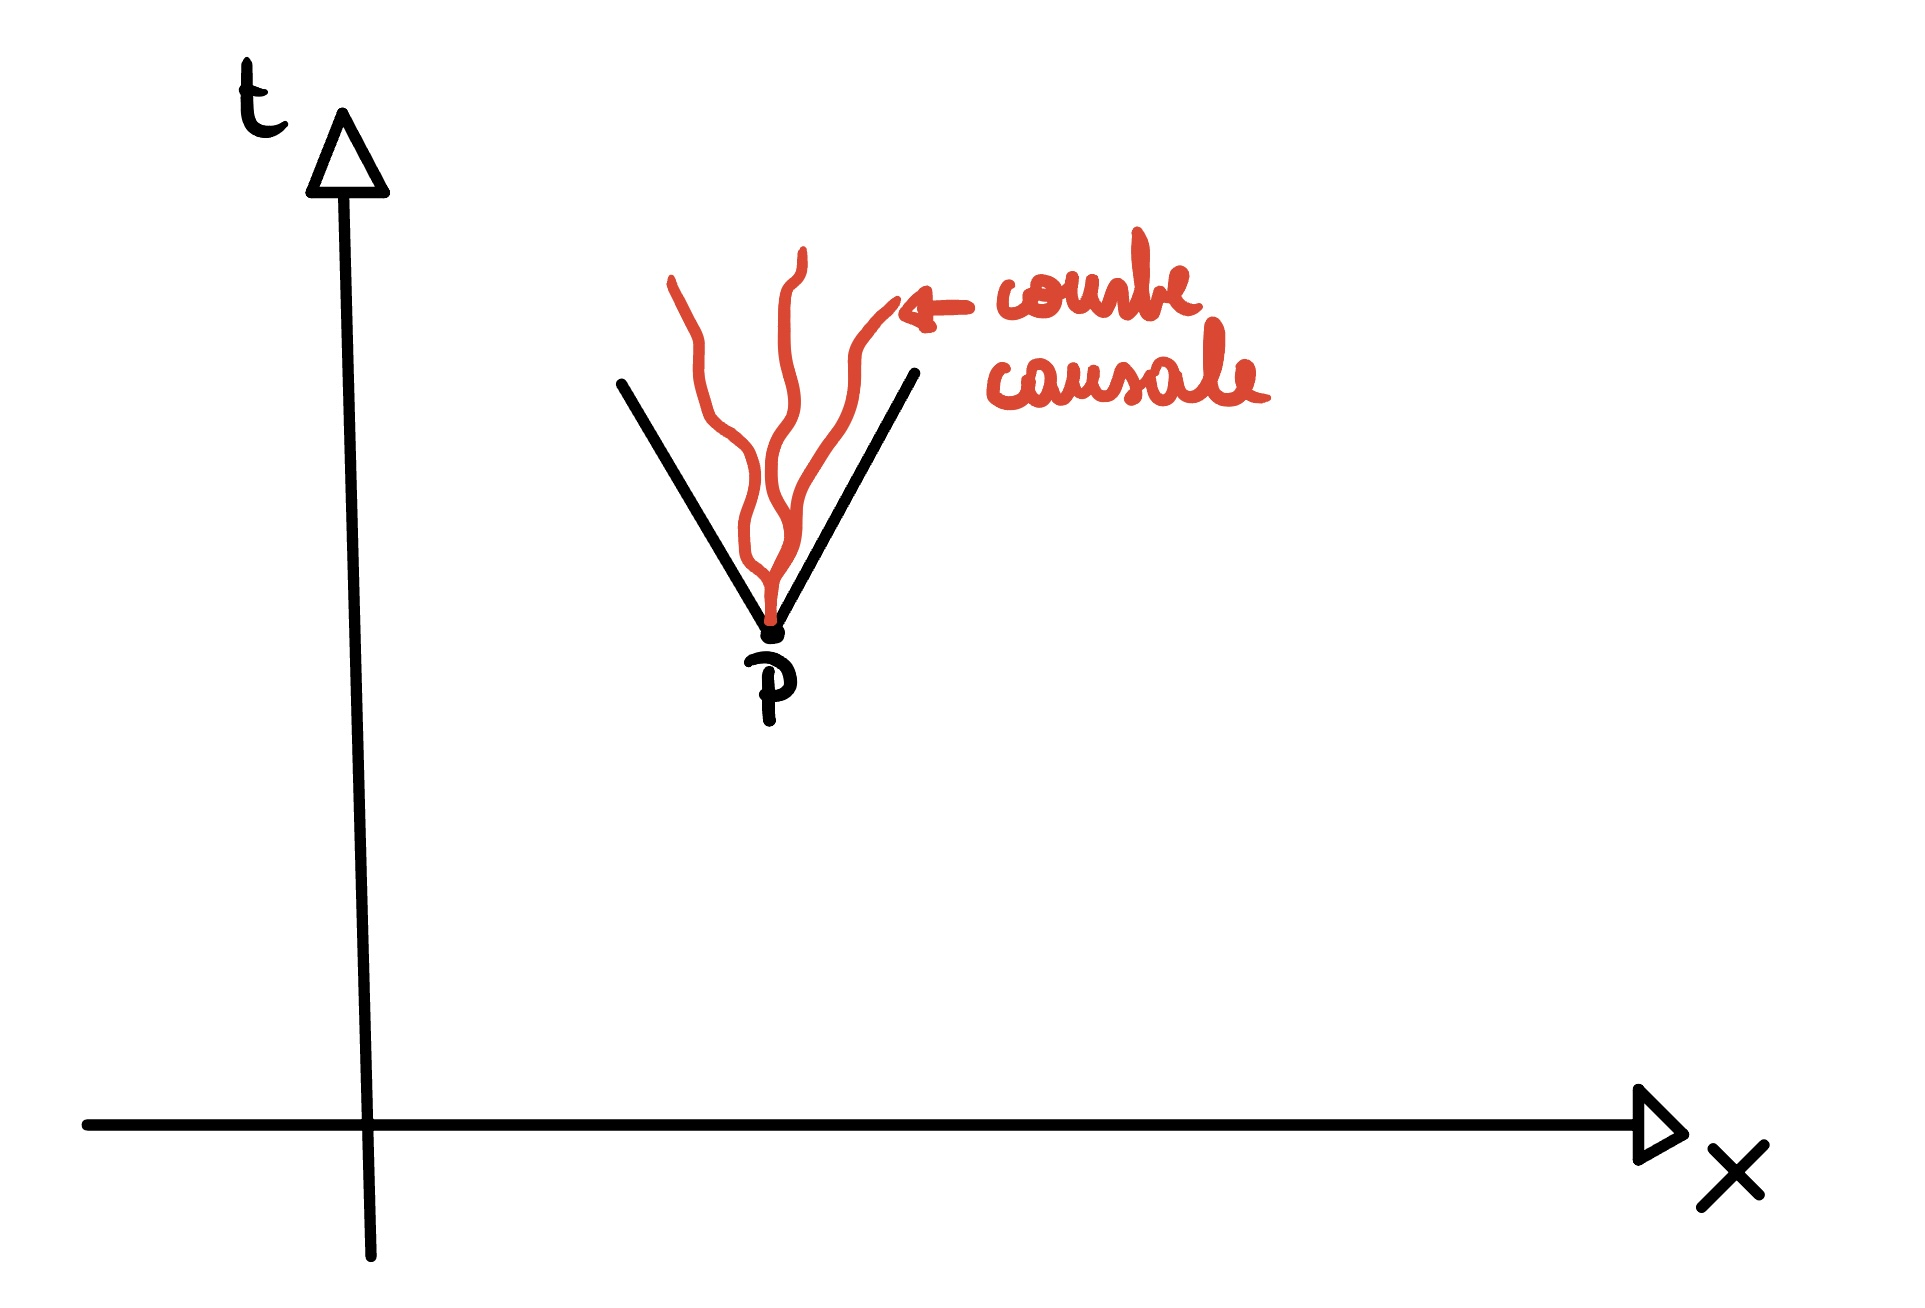
\includegraphics[width=0.5\linewidth]{Chapitres/2. Relativité Restreinte/Images/exemple1.jpg}
    \caption{}
    \label{fig:2.6}
\end{figure}
\end{exmp}

    \begin{exmp}
    Si $\mathcal{S}$ est la trajectoire d'un observateur inertiel au repos (une droite dans $\R^{1,3}$), alors $I^{+}(\mathcal{S}) = J^{+}(\mathcal{S}) = \R^{1,3}$ tout entier.
    \begin{figure}[H]
        \centering
        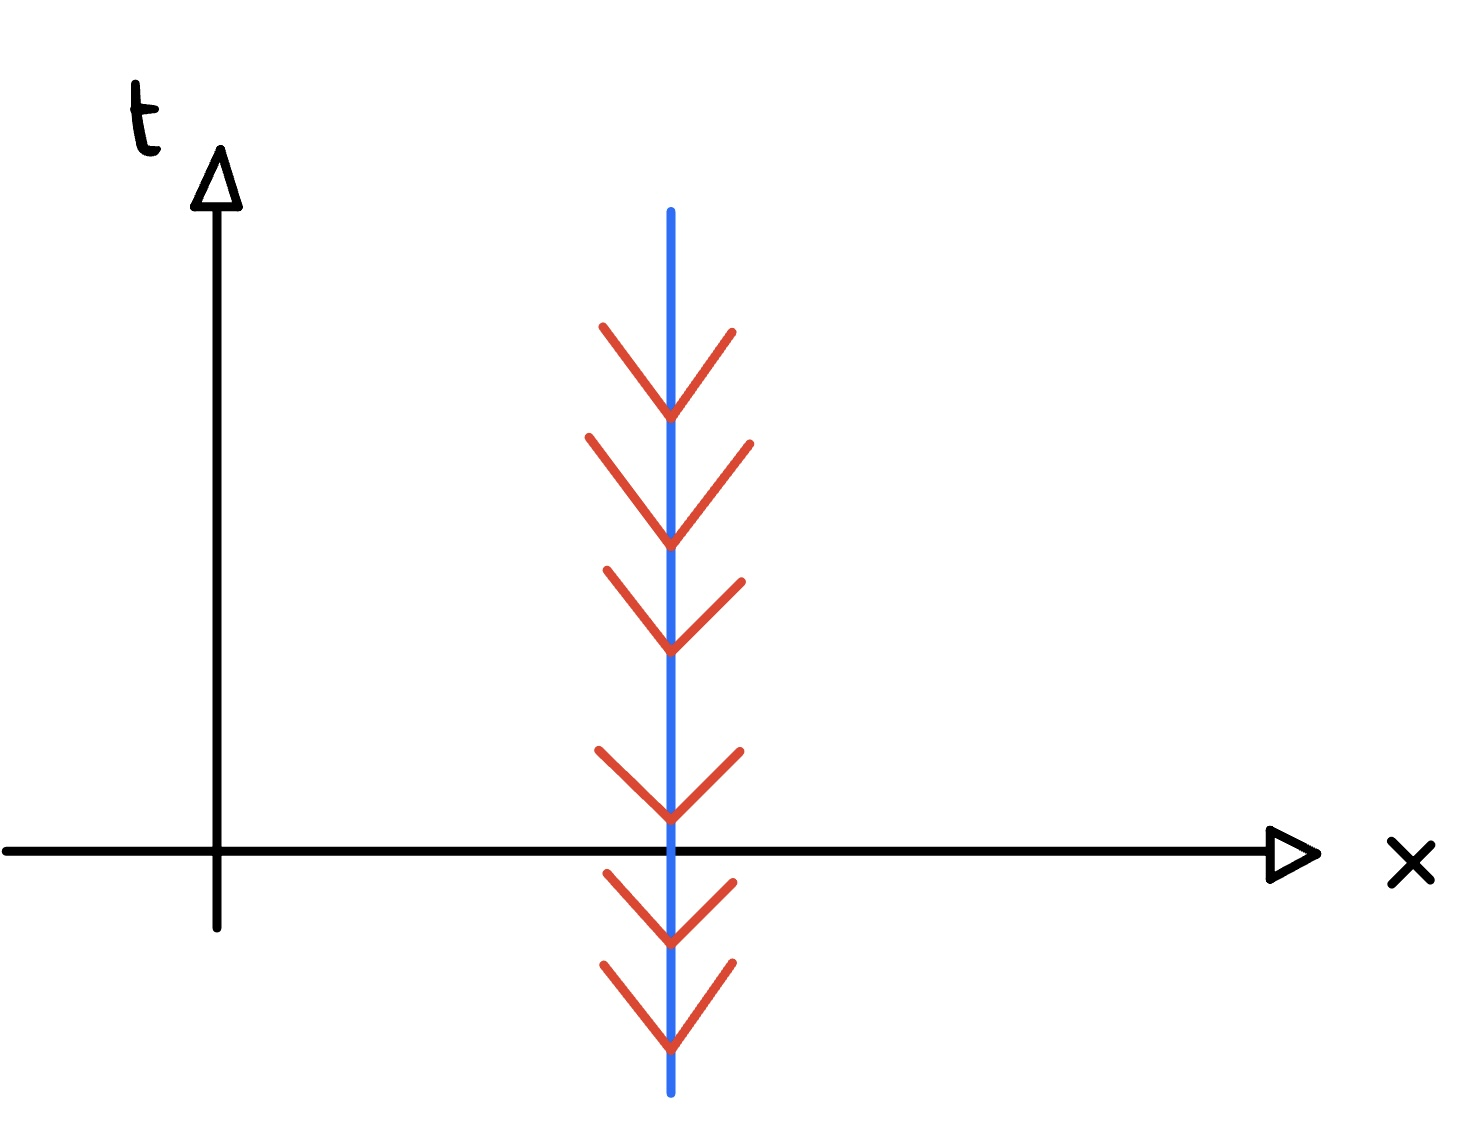
\includegraphics[width=0.5\linewidth]{Chapitres/2. Relativité Restreinte/Images/exemple2.jpg}
        \caption{}
        \label{fig:2.7}
    \end{figure}
\end{exmp}
Intéressons-nous à un dernier exemple fondamental : l'expérience de Rindler.

\subsection{L'expérience de Rindler}
Considérons maintenant le cas d'un observateur accéléré uniformément\footnote{Vous pouvez également consulter la \href{https://youtu.be/yyzPCtmll58?si=rmU0qF_0cyaDOqnC}{vidéo d'Eigenchris} sur ce sujet.}. 
\begin{theoremframe}
    \begin{propri}
        Soit une courbe de genre temps $x^\alpha(\lambda)$ et son champ de vecteurs tangents. Il existe toujours une paramétrisation de la courbe telle que la norme du champ tangent est normalisée : 
        \begin{equation}
            v^\alpha v_\alpha = -1
        \end{equation}
        De plus, cette paramétrisation est le temps propre de la courbe.
    \end{propri}
\end{theoremframe}
\begin{proof}
    La norme du champ tangent pour une paramétrisation arbitraire est
    \begin{equation}
        \eta_{\alpha\beta} \, \frac{\td x^\alpha}{\td \lambda} \frac{\td x^\beta}{\td \lambda} = - \alpha^2(\lambda) < 0
    \end{equation}
    Où $\alpha$ est une fonction arbitraire de la paramétrisation. Effectuons le changement de variable $\lambda \to \mu $ :
    \begin{equation}
        \eta_{\alpha\beta} \, \frac{\td x^\alpha}{\td \mu} \frac{\td x^\beta}{\td \mu} \lt \frac{\td \mu}{\td \lambda} \rt^2 = - \alpha^2 (\lambda (\mu))
    \end{equation}
    Il suffit alors de choisir $\mu(\lambda)$ tel que
    \begin{equation}
        \lt \frac{\td \mu}{\td \lambda} \rt^2 = \alpha^2 (\lambda)
    \end{equation}
    De plus, infinitésimalement, on obtient dans ces variables
    \begin{equation}
        - \td \mu ^2 = \eta_{\alpha\beta} \, \td x^\alpha \td x^\beta
    \end{equation}
    Le côté droit de cette équation est exactement $\td s^2 = - \td \tau^2$. La paramétrisation $\mu$ choisie est donc simplement le temps propre $\tau$ de la courbe.
\end{proof}
Soit une particule suivant une courbe $x^\alpha$ paramétrisée par son temps propre. On définit la quadri-vitesse comme :
\begin{equation}
    v^\alpha \equiv \frac{\td x^\alpha}{\td \tau}
\end{equation}
où $v^{\alpha} v_{\alpha} = -1$ en vertu de la propriété précédente. La 4-accélération est définie par :
\begin{equation*}
    a^{\alpha} \equiv \frac{\td v^{\alpha}}{\td \tau}
\end{equation*}
Nous souhaitons étudier la trajectoire d'un observateur à accélération constante, donc avec la condition 
\begin{equation*}
    a_{\alpha}a^{\alpha} = a^{2} = \text{cste}
\end{equation*}
Choisissons un référentiel tel que l'accélération se fait dans la direction $x^{1}$ et décrit un mouvement dans le plan $(x^{0}, x^{1})$. Nous supposerons que $v^2 = v^3 = 0$. Les équations du mouvement pour cet observateur accéléré sont
\begin{align}
    \begin{dcases}
        \dfrac{\td x^{\alpha}}{\td \tau} = v ^{\alpha}\\
        \dfrac{\td v^{\alpha}}{\td \tau} = a^{\alpha}
    \end{dcases}
\end{align}
muni des conditions
\begin{align}
    v^{\alpha}v_{\alpha} & = -1 = -(v^{0})^2 + (v^{1})^2\\
    a^{\alpha}a_{\alpha} & = a^2 = -(a^{0})^2 + (a^{1})^2 = \mathrm{cste}
\end{align}

Or, comme $v^{\alpha}v_{\alpha} = -1$:

\begin{align}
    \frac{\td v^\alpha v_\alpha}{\td \tau} &= 2 a^{\alpha}v_{\alpha} = 0 \\
    \implies &-a^{0}v^{0} + a^{1}v^{1} = 0\\
    \label{eq:2.57}
    \implies &v^{1} = \frac{v^{0}a^{0}}{v^{1}}
\end{align}

En adoptant temporairement des indices covariants pour améliorer la lisibilité (notons que comme seul des carrés interviennent, cela ne change rien aux calculs) :
\begin{align}
    a_1^2 &= 1 \cdot a_1^2\\
    &= \lt v_0^2 - v_{1}^2 \rt a_{1}^2\\
    &= v_{0}^2 \lt 1 - \frac{a_0^2}{a_1^2} \rt a_1^2\\
    &= v_{0}^2(a_{1}^2 - a_{0}^2)\\
    &= v_{0}^2 a^2
\end{align}
Nous obtenons donc que $a^1 = av^{0}$ et que $a^0 = av^{1}$ par \ref{eq:2.57}. Ce problème peut se réécrire en forme matricielle comme:
\begin{equation}
\frac{\td }{\td \tau} \begin{pmatrix}
    v^0 \\
    v^1
\end{pmatrix} = \begin{pmatrix}
    0 & a \\
    a & 0
\end{pmatrix}
\begin{pmatrix}
    v^0 \\
    v^1
\end{pmatrix}
\end{equation} 
La solution de ce système est
\begin{align} 
    \begin{dcases}
        v^{0} = \cosh{a\tau}\\
        v^{1} = \sinh{a\tau}
    \end{dcases}
\end{align}
Et la position est donc donné par
\begin{align} 
\label{eq:Rindler}
    \begin{dcases}
        x^{0} = \frac{1}{a}\sinh{a\tau}\\
        x^{1} = \frac{1}{a}\cosh{a\tau}
    \end{dcases}
\end{align}
À quoi ressemble cette trajectoire graphiquement ? On a que:
\begin{align}
    &v^{1} = 0|_{\tau = 0}\\
    &(x^1)^2 - (x^0)^2 = \frac{1}{a^2}
\end{align}
il s'agit donc d'une branche d'hyperbole.
\begin{figure}[H]
    \centering
    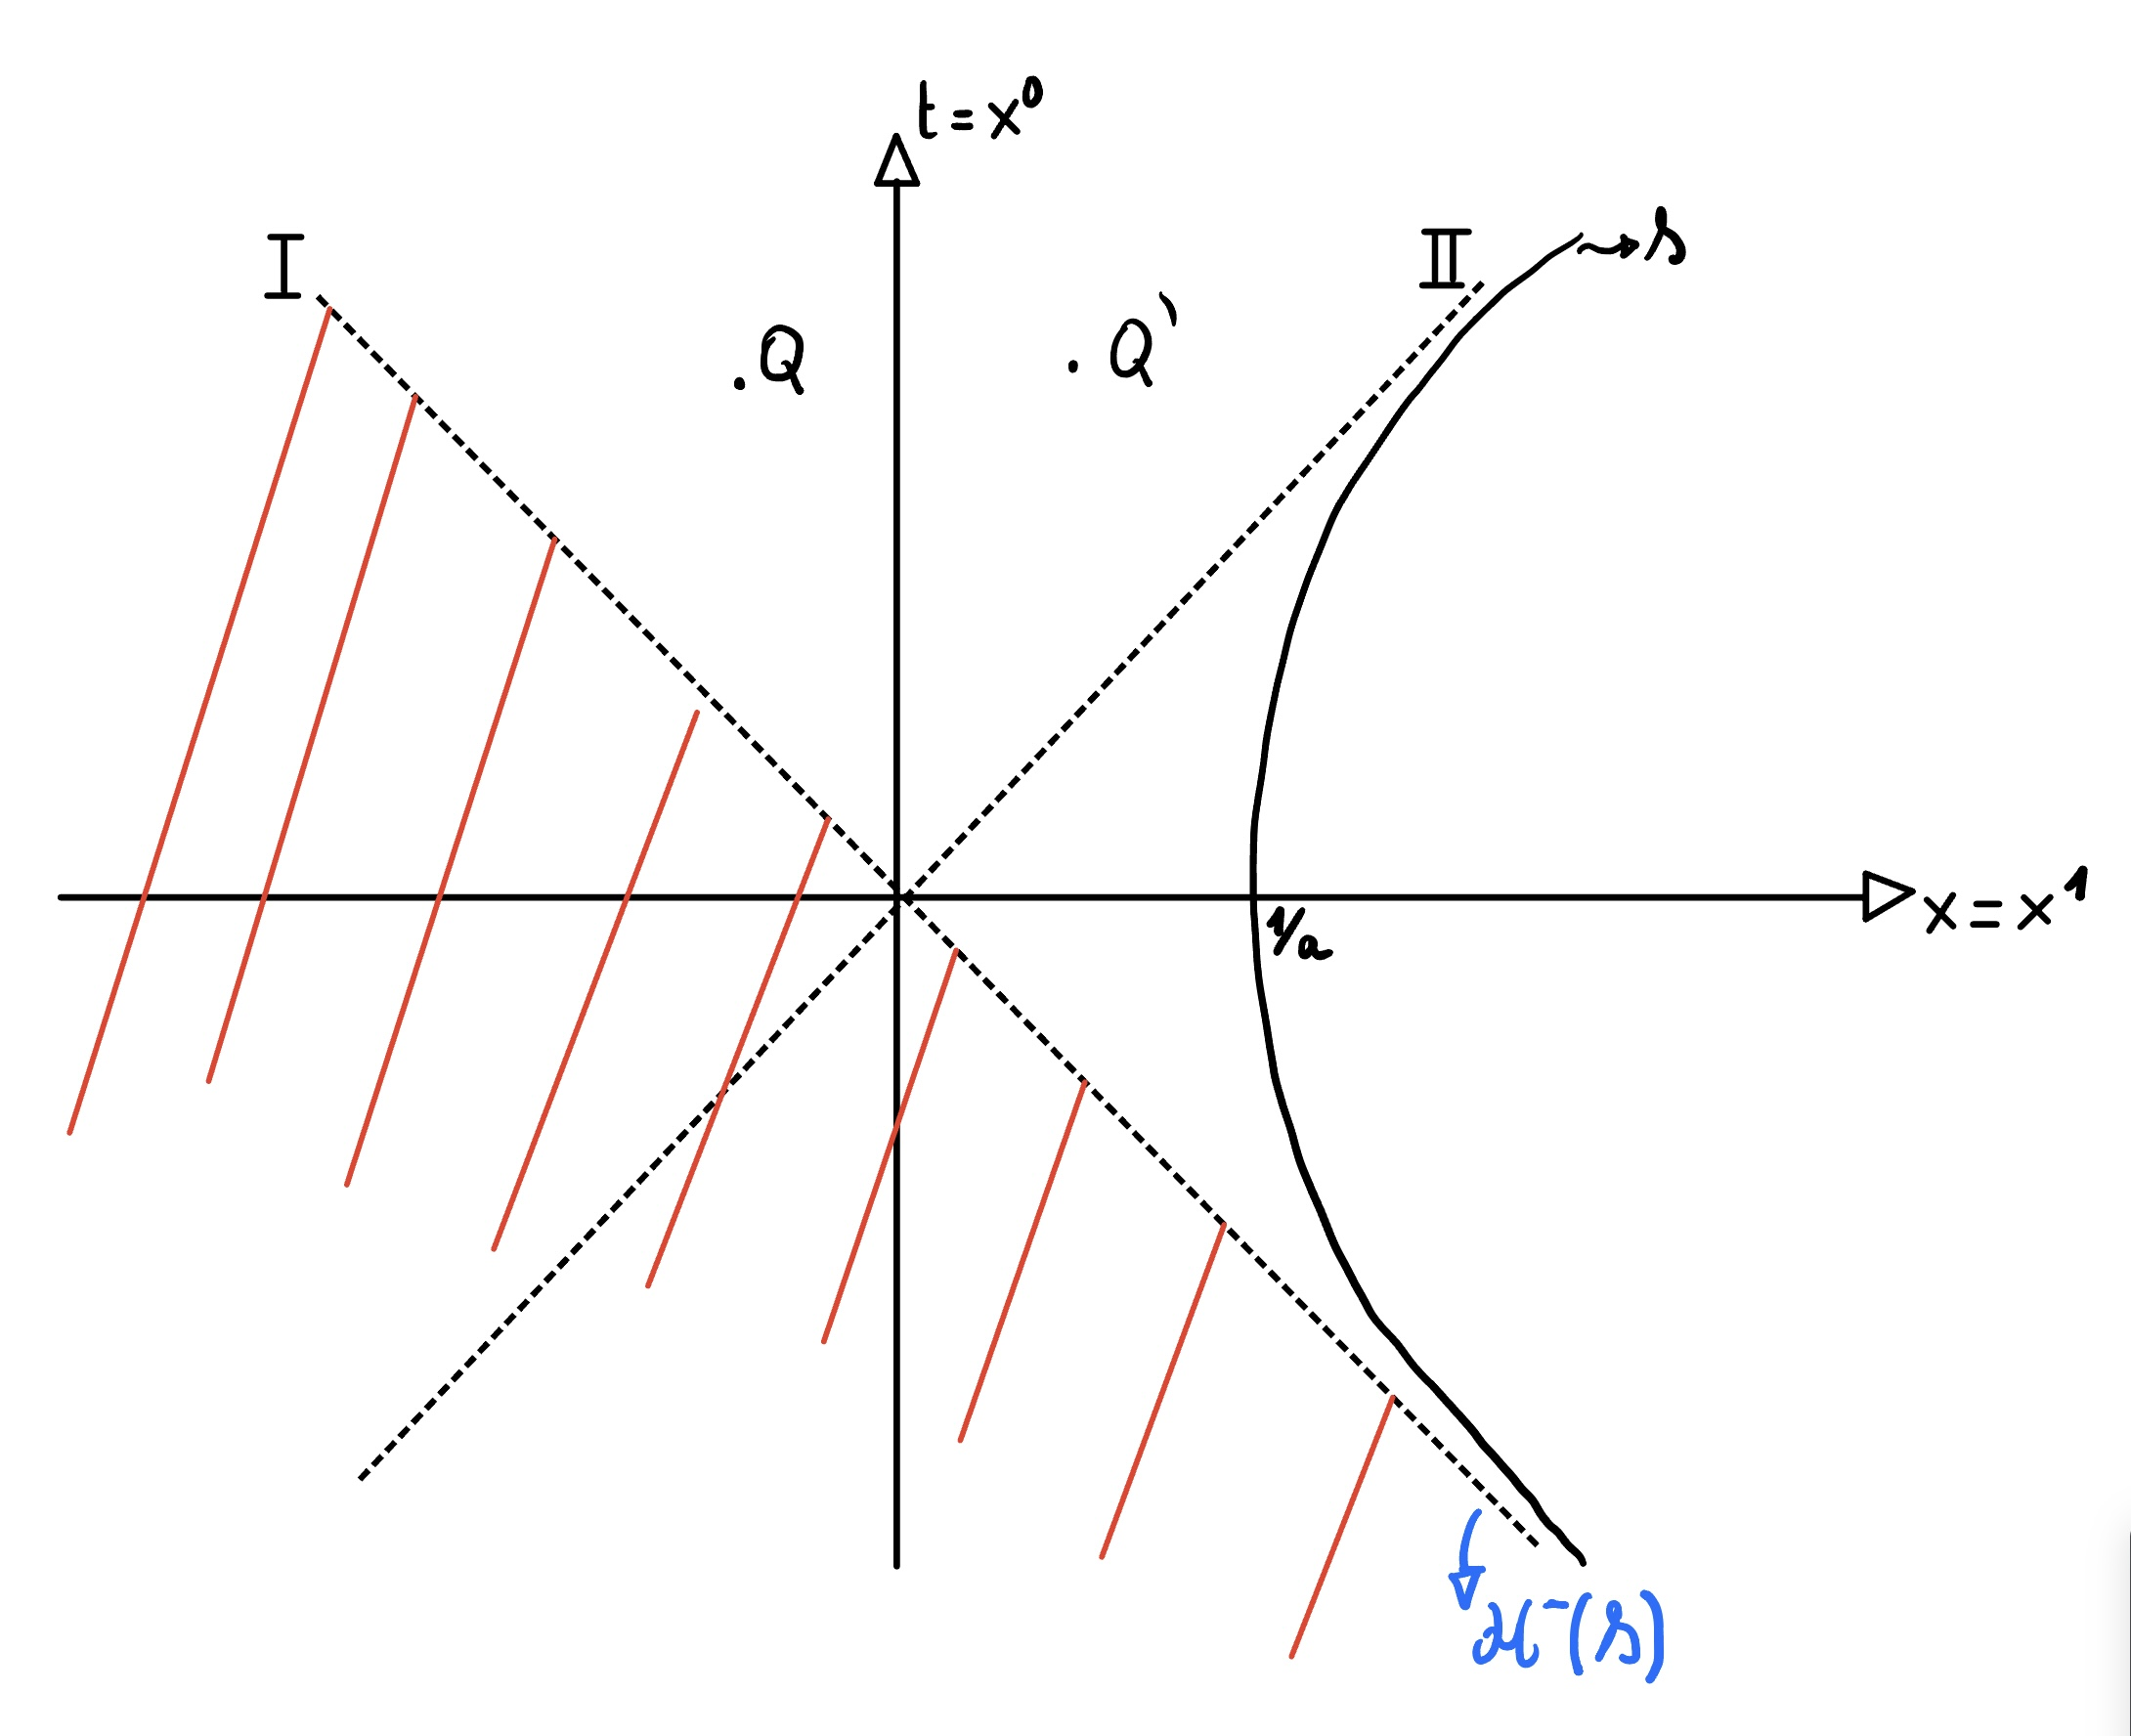
\includegraphics[width=0.5\linewidth]{Chapitres/2. Relativité Restreinte/Images/Courbe hyperbole 1.jpg}
    \caption{}
    \label{fig:2.8}
\end{figure}

Cette ensemble de points $\mathcal{S}$ est la trajectoire d'un observateur accéléré dans l'espace-temps de Minkowski. Quelques remarques:
\begin{enumerate}
    \item $\mathcal{S}$ ne pourra jamais influencer ce qui se trouve sous la ligne de lumière \cRM{1} (indiqué en rouge sur la figure \ref{fig:2.8}). 

    \item $I^{+}(\mathcal{S})$ est l'ensemble des évènements que la trajectoire $\mathcal{S}$ peut influencer, et correspond à la zone non hachurée de la figure \ref{fig:2.8}.

    \item La frontière de $I^{+}(\mathcal{S})$ est l'horizon des événements passé de $\mathcal{S}$. $\mathcal{H}^{+}(\mathcal{S}) = \cRM{1}$ est la frontiére de l'horizon des événements passé. 
\end{enumerate}



La frontière de $\cRM{1}^{+}(\mathcal{S})$ est l'horizon des événements passé de $\mathcal{S}$. $\mathcal{H}^{+}(\mathcal{S}) = \cRM{1}$ est la frontiére de l'horizon des événements passé. 

\begin{center}
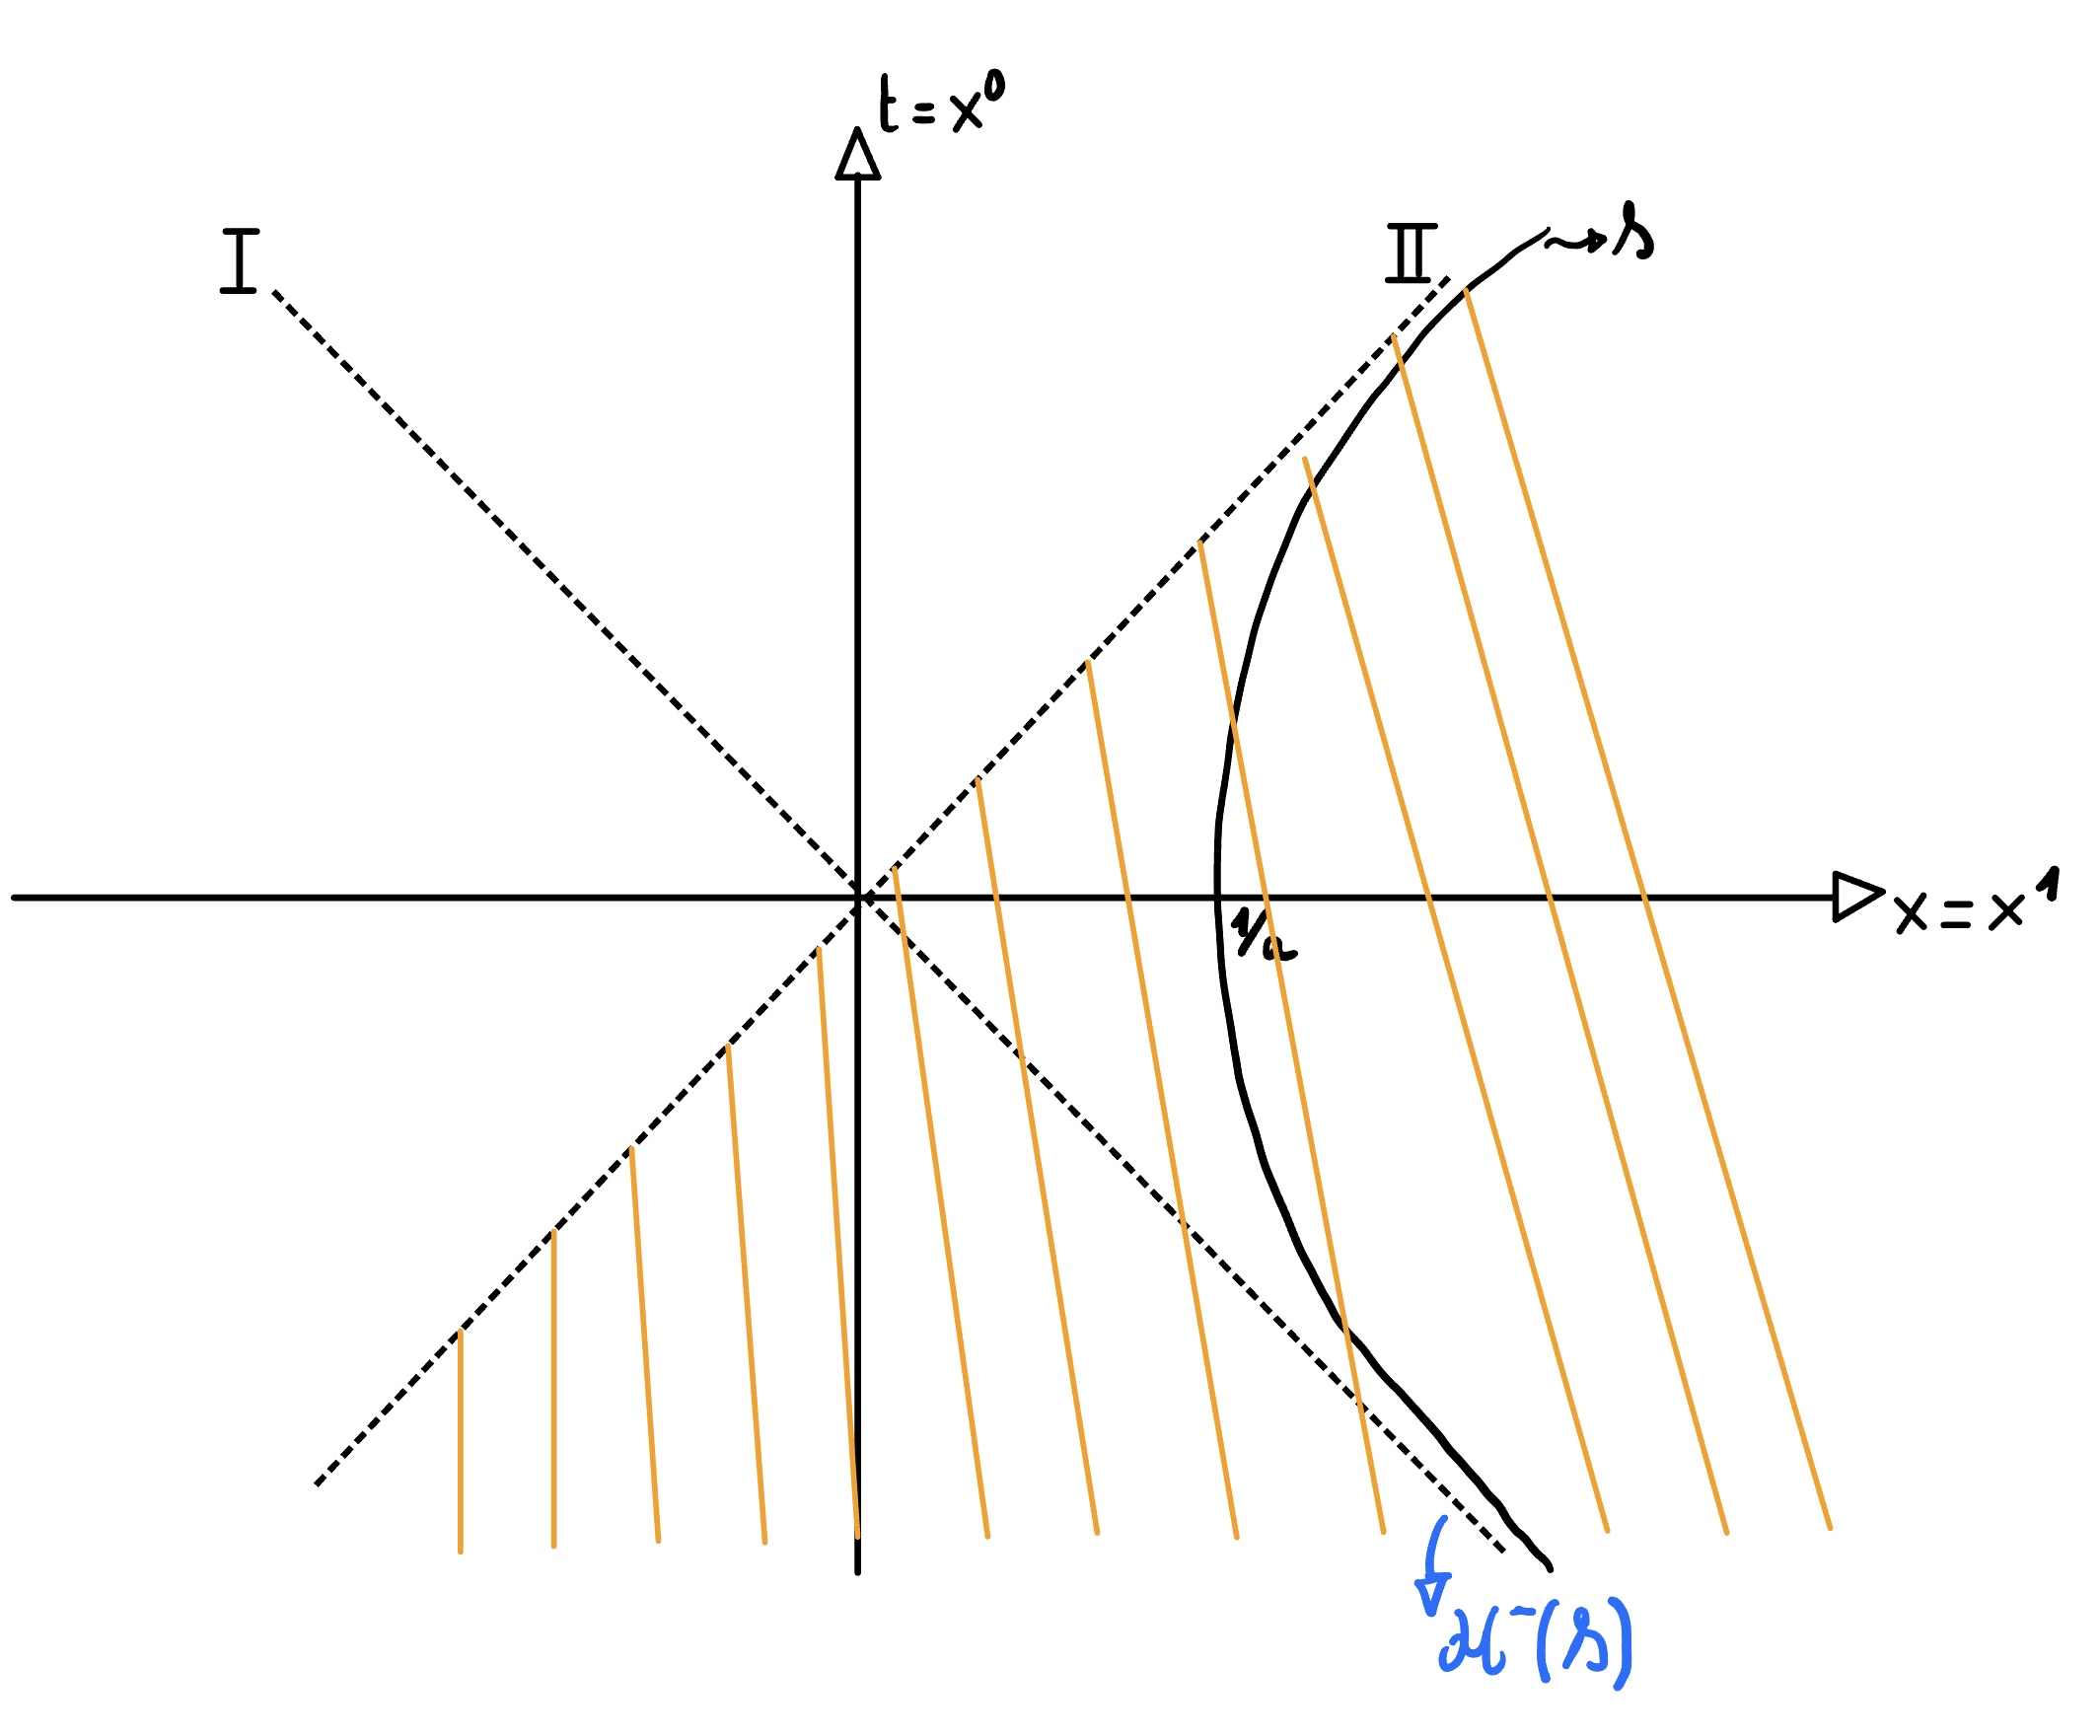
\includegraphics[scale=0.1]{Chapitres/2. Relativité Restreinte/Images/Courbe hyperbole 2.jpg}
\label{Parabolique 2}
\end{center}

$\cRM{1}^{-}(\mathcal{S})$ est une zone où la trajectoire $\mathcal{S}$ peut être affecté par les événements qui ont lieu dans la zone hachurée pour la graphique \ref{Parabolique 2}. 

La frontière de $\cRM{1}^{-}(\mathcal{S})$ est l'horizon des événements futur  de $\mathcal{S}$. Qu'on note $\mathcal{H}^{-}(\mathcal{S})$.
\subsection{Le référentiel de Rindler*}
Illustrons à présent le lien entre référentiels et géométrie. Supposons que nous souhaitons nous placer dans le référentiel de l'observateur non-inertiel de Rindler, dont le changement de coordonnées est donné à partir de l'équation \ref{eq:Rindler} par\footnote{Pour une dérivation de ces coordonnées (et une étude plus détaillée), consultez la \href{https://youtu.be/O92pQXZaEnw}{vidéo d'Eigenchris} sur ce sujet.}
\begin{align}
    \begin{dcases}
        t = \tilde x \sinh (\alpha \tilde t) \\
        x = \tilde x \cosh (\alpha \tilde t)
    \end{dcases}
\end{align}
où $(\tilde t, \tilde x)$ sont les coordonnées du point de vue d'un observateur accéléré à accélération constante $\alpha$ (et dont l'horizon se trouve à l'origine). La transformation inverse est donnée par :
\begin{align}
    \begin{dcases}
        \tilde t = \frac{1}{\alpha} \, \mathrm{artanh}\lt \frac{t}{x} \rt \\
        \tilde x = \sqrt{t^2 - x^2}
    \end{dcases}
\end{align}
En différenciant et en injectant ces équations dans la métrique de Minkowski, on obtient
\begin{equation}
    \td s^2 = - (\alpha \tilde x)^2 \td \tilde t^2 + \td \tilde x^2 + \td \tilde y^2 + \td \tilde z^2
\end{equation}
Le changement d'un référentiel inertiel vers le référentiel hyperbolique a donc modifié la métrique $\eta_{\mu\nu}$ dans ces coordonnées, qui dépendra explicitement des coordonnées : $\tilde \eta_{\mu\nu} = \mathrm{diag} (-(\alpha \tilde x)^2, 1, 1,1)$.
\begin{exmp}
    Sous l'action d'une rotation d'angle $\Omega$ autour de l'axe $z$, la métrique de Minkowski devient
    \begin{equation}
        \td s^2 = -\ltc c^2 - \Omega^2 (x'^2 + y'^2) \rtc \td t^2 + \td x'^2 +\td y'^2 + \td z'^2 - 2\Omega \,y' \td x \, \td t + 2\Omega\, x' \td y'\, \td t
    \end{equation}
    Ou, en terme de la métrique :
    \begin{align}
        \eta'_{\mu\nu} = \begin{pmatrix}
            - c^2 + \Omega^2 (x'^2 + y'^2) & - \Omega \, y' & \Omega \, x' & 0 \\
            - \Omega \, y' & 1 & 0 & 0\\
            \Omega \, x' & 0 & 1 & 0\\
            0 & 0 & 0 & 1
        \end{pmatrix}
    \end{align}
\end{exmp}
\cutebreak
De manière générale, dans un référentiel arbitraire (possiblement non-inertiel), l'intervalle s'écrit comme une forme quadratique :
\begin{equation}
    \td s^2 = g_{\mu\nu}\, \td x^\mu \, \td x^\nu
\end{equation}
L'intervalle (et donc la métrique) caractérisent la notion de \emph{distance} de l'espace-temps, et sont donc des propriétés de la géométrie de l'espace-temps considéré. Bien qu'ils dépendent du référentiel considéré, on peut toute fois extraire des quantités \emph{intrinsèques} à la géométrie considérée, donc indépendantes du référentiel. Un exemple d'une telle quantité sera la \emph{courbure}. 
\section{Hypersurfaces de Cauchy*}
La notion d'hypersurface de Cauchy est importante afin que les problèmes aux limites soient bien posés\footnote{Selon Hadamard :)}.

\begin{theoremframe}
    \begin{defi}
        Le \textit{domaine de dépendance future} (ou \textit{développement futur}) d'une région $\mathcal{S}$ de l'espace-temps est l'ensemble des points $P \in \R^{1,3}$ tels que \emph{toute} courbe causale passant par $P$ intersecte $\mathcal{S}$. Il est noté $\mathcal{D}^+(\mathcal{S})$.
    \end{defi}
\end{theoremframe}
\begin{exmp}
    Soit $\mathcal{S} = $ un segment de droite à $t = \text{ cste}$ (voir Schéma). $P \in \mathcal{D}^+(\mathcal{S})$ (car toute courbe causale passe nécessairement par $\mathcal{S}$), mais $Q \notin \mathcal{D}^+(\mathcal{S})$ (car il existe des courbes causales ne passant pas par $\mathcal{S}$).
\end{exmp}
La frontière future (bord) de $\mathcal{D}^+(\mathcal{S})$, notée $\mathcal{H}^+(\mathcal{S})$, est appelée \emph{horizon de Cauchy} de $\mathcal{S}$. Ce qui se passe en $P \in \mathcal{D}^+(\mathcal{S})$ est complètement déterminé par ce qui s'est passé en $\mathcal{S}$. Plus généralement, connaissant ce qui s'est passé en $\mathcal{S}$, on ne peut prédire complètement ce qui se passera \emph{que} pour les événements de $\mathcal{D}^+(\mathcal{S})$.

\begin{rmk}
    $\mathcal{D}^+(\mathcal{D}^-(\mathcal{S})) \neq \mathcal{S}$ : il existe des points (voir Q dans schéma précédent) qui n'appartiennent pas à $\mathcal{D}^-(\mathcal{S})$ mais qui peuvent influencer $\mathcal{S}$. Autrement dit, connaître tout de $\mathcal{D}^-(\mathcal{S})$ ne suffit pas à tout connaître de $\mathcal{S}$.
\end{rmk}

\begin{theoremframe}
    \begin{defi}
        Un \emph{ensemble acausal} est un ensemble $\mathcal{A}$ tel que $\forall P, Q \in \mathcal{A}$, l'intervalle $(\Delta s_{PQ})^2$ est de genre espace.
    \end{defi}
\end{theoremframe}
\begin{theoremframe}
    \begin{defi}
        Une \emph{hypersurface de Cauchy} est une hypersurface acausale sans bord $\mathcal{S}$ telle que
        \begin{align}
            \mathcal{D}(\mathcal{S}) \equiv \mathcal{D}^+(\mathcal{S}) \cup \mathcal{D}^-(\mathcal{S}) = \R^{1,3}
        \end{align}
    \end{defi}
\end{theoremframe}
Si on connait complètement une hypersurface de Cauchy, on peut prédire tout ce qui se passera, et on peut reconstruire tout ce qui s'est passé. On peut déterminer, à l'aide de la dynamique (des équations du mouvement) de la théorie considérée (contrainte par le fait que tout signal se propage à vitesse $v \leq c$), l'état de l'espace-temps tout entier à partir de l'information spécifiée sur $\mathcal{S}$. Comme en outre, l'hypersurface est acausale, ses divers évènements sont indépendants : il n'y a pas de redondance d'information.

\begin{rmk}
    Un espace-temps possédant une hypersurface de Cauchy est dit \emph{globalement hyperbolique}. Par exemple, l'espace-temps plat de Minkowksi en est un. D'autres ne le sont pas, et nécéssitent de fixer des conditions au bord, comme par exemple l'espace Anti-de Sitter (AdS).
\end{rmk}
}